\documentclass[a4paper,twoside,openright,12pt,slovene]{book}
\usepackage[pdftex]{./Izgled/UNI-LJ-FE-Diploma} % stil zaključnega dela UL FE
\usepackage[utf8]{inputenc} % predloga uporablja standardno kodiranje Unicode UTF-8, ki podpira šumnike
\usepackage[greek,english,slovene]{babel} % seznam uporabljenih jezikov (zadnji na seznamu je primarni)
\usepackage{amsfonts}
\tolerance=2000

% PDF/A %%%%%%%%%%%%%%%%%%%%%%%%%%%%%%%%%%%%%%%%%%%%%%%%%%%%%%%%%%%%%%%%%%%%%%%%%%%%%%%%%%%%%%%%%%%%%%%%%%%%%%%%%%%%%%%%
\usepackage{filecontents}
\begin{filecontents*}{\jobname.xmpdata}
    \Title{Kontekstualiziran priporočilni sistem za dnevne aktivnosti starejših} % Mora biti enak kot je v prijavi teme!
    \Author{Gašper Leskovec}
\end{filecontents*}
\usepackage[a-1b]{pdfx}
%%%%%%%%%%%%%%%%%%%%%%%%%%%%%%%%%%%%%%%%%%%%%%%%%%%%%%%%%%%%%%%%%%%%%%%%%%%%%%%%%%%%%%%%%%%%%%%%%%%%%%%%%%%%%%%%%%%%%%%%

% LaTeX PAKETI %%%%%%%%%%%%%%%%%%%%%%%%%%%%%%%%%%%%%%%%%%%%%%%%%%%%%%%%%%%%%%%%%%%%%%%%%%%%%%%%%%%%%%%%%%%%%%%%%%%%%%%%%

% Dodatni simboli
\usepackage{textcomp}                               % dodatni simboli (kot npr. €)
\usepackage{gensymb}                                % dodatni simboli \de­gree, \cel­sius, \pert­hou­sand, \mi­cro, \ohm
\newcommand{\uppi}{\textrm{\greektext p\latintext}} % velika grška črka P z \uppi, alternativa simbolu \Pi

% Osnovno oblikovanje
\hypersetup{unicode,hidelinks,breaklinks,hyperindex} % dodatne možnosti hiperpovezav
\usepackage[normalem]{ulem}                          % podčrtavanje in prečrtavanje teksta
\usepackage{float}                                   % dodatne možnosti oblikovanja objektov
\usepackage{enumitem}                                % dodatne možnosti oblikovanja seznamov
\usepackage{booktabs}                                % lepe horizontalne črte v tabelah

% Dodatno oblikovanje
\usepackage{longtable}      % večstranske tabele
\usepackage{caption}        % dodatne možnosti označevanja objektov

% Matematična orodja
\usepackage{mathtools} % http://mirrors.ctan.org/macros/LaTeX/contrib/mathtools/mathtools.pdf
\usepackage{bm}        % ukaz za odebeljeni tisk \bm v matematičnih okoljih

% Grafična orodja
\usepackage{graphicx}                 % vključevanje bitnih slik z ukazom \includegraphics
\usepackage{grffile}                  % podpora presledkom pri ukazu \includegraphics
\usepackage{tikz}
\usetikzlibrary{arrows.meta, positioning}

% Vključevanje datotek
\usepackage{pdfpages} % vključevanje PDF datotek z ukazom \includegraphics
\usepackage{epstopdf} % vključevanje EPS datotek z ukazom \includegraphics
\usepackage{listings} % orodja za izpisovanje programske kode
\lstset{              % nastavitve orodja za izpisovanje programske kode
    basicstyle=\ttfamily\footnotesize,
    breaklines=true,
    numbers=left,
    numberstyle=\scriptsize,
    keywordstyle=\color{blue},
    commentstyle=\color{unilj},
    stringstyle=\color{olive},
}
%%%%%%%%%%%%%%%%%%%%%%%%%%%%%%%%%%%%%%%%%%%%%%%%%%%%%%%%%%%%%%%%%%%%%%%%%%%%%%%%%%%%%%%%%%%%%%%%%%%%%%%%%%%%%%%%%%%%%%%%

% DEKLARACIJE %%%%%%%%%%%%%%%%%%%%%%%%%%%%%%%%%%%%%%%%%%%%%%%%%%%%%%%%%%%%%%%%%%%%%%%%%%%%%%%%%%%%%%%%%%%%%%%%%%%%%%%%%%
\naslov{Kontekstualiziran priporočilni sistem za dnevne aktivnosti starejših} 
\avtor{Gašper Leskovec} 
\mentor{prof. dr. Andrej Košir}
\date{Ljubljana, \the\year}
\univerza{Univerza v Ljubljani}
\definecolor{unilj}{cmyk}{0.00, 0.94, 0.94, 0.06} % barva Univerze v Ljubljani

\delo{Magistrsko delo\\~\\Magistrski študijski program druge stopnje Elektrotehnika}
\fakulteta{Fakulteta za elektrotehniko}

% DOKUMENT %%%%%%%%%%%%%%%%%%%%%%%%%%%%%%%%%%%%%%%%%%%%%%%%%%%%%%%%%%%%%%%%%%%%%%%%%%%%%%%%%%%%%%%%%%%%%%%%%%%%%%%%%%%%%
\begin{document}
\frontmatter

\selectlanguage{slovene}

%******************************* NASLOVNICA ************************************
\maketitle

%******************************* ZAHVALA ***************************************
\zahvala
Pri magistrskem delu se zahvaljujem mentorju prof. dr. Andreju Koširju za strokovno vodenje, jasne usmeritve ter konstruktivne komentarje pri načrtovanju in izvedbi eksperimentov. Posebna zahvala gre družini in prijateljem za podporo in razumevanje v času nastajanja magistrskega dela.

%******************************* POVZETEK IN KLJUČNE BESEDE ********************
\povzetek
Magistrsko delo obravnava priporočanje kombinacij dnevnih
aktivnosti starejšim uporabnikom. Ocene 6\,579 kombinacij ene do treh
aktivnosti za 679 uporabnikov so izračunane po pravilu iz vprašalniških
odgovorov, uporabniških uteži in združljivosti aktivnosti. Napoveduje jih
matrična faktorizacija (SVD, knjižnica Surprise), časovni in prostorski
kontekst pa upoštevamo z naknadnim filtriranjem kandidatnih kombinacij.

Na odloženem testnem delu (25~\% od 3\,053\,029 ocen) SVD doseže
RMSE $0{,}0819$ in MAE $0{,}0531$. Pri izboru petih kombinacij brez
konteksta doseže F1-mero $0{,}339$ (z upoštevanjem izenačenih ocen
$0{,}982$), razvrščanje po popularnosti pa $0{,}151$ ($0{,}531$).
Pri strogem kontekstnem filtru priporočila prejme 608 uporabnikov
(89,5~\%). Pri 398 uporabnikih z več kot petimi skladnimi kombinacijami
znaša F1-mera s kontekstno referenco $0{,}700$, pri popularnosti $0{,}569$,
pri naključnem rangiranju pa $0{,}285$. Utežene F1-mere skupin kontekstov
M3--M5 so med $0{,}623$ in $0{,}698$. Rezultati merijo ujemanje
z izračunanimi ocenami.


\kljucnebesede
priporočilni sistemi, sodelovalno filtriranje, matrična faktorizacija, SVD, kontekstno priporočanje, starejši uporabniki


\selectlanguage{english}

%******************************* ABSTRACT AND KEYWORDS *************************

\abstract
This thesis investigates recommendations of daily activity
combinations for elderly users. Ratings of 6,579 combinations of one to
three activities for 679 users are computed by a rule from questionnaire
answers, user weights and activity compatibilities. They are predicted by
matrix factorization (SVD, Surprise library), while temporal and spatial
context is incorporated through post-filtering of candidate combinations.

On a held-out test set (25\% of 3,053,029 ratings) SVD achieves an RMSE of
0.0819 and an MAE of 0.0531. When selecting five combinations without
context it achieves an F1-score of 0.339 (0.982 with ties), compared with
0.151 (0.531) for popularity ranking. Under the strict context filter, 608
users (89.5\%) receive recommendations. For the 398 users with more than
five feasible combinations, the F1-score with the context-filtered reference
is 0.700, compared with 0.569 for popularity and 0.285 for random ranking.
User-weighted F1-scores of the context groupings M3--M5 range from 0.623 to
0.698. The results measure agreement with the computed ratings.


\keywords
recommender systems, collaborative filtering, matrix factorization, SVD, context-aware recommendation, elderly users


\selectlanguage{slovene}

%******************************* KAZALO ****************************************
\tableofcontents

%******************************* SEZNAM SLIK, SEZNAM TABEL *********************
\seznamslik
\seznamtabel

%******************************* SEZNAM SIMBOLOV *******************************
\seznamsimbolov
\begin{itemize}[leftmargin=*,itemsep=2pt]
  \item[$u$] uporabnik (identifikator uporabnika)
  \item[$i$] priporočilni element: kombinacija od ene do treh aktivnosti
  \item[$c$] kontekst (npr.\ časovni in prostorski kontekst)
  \item[$r_{u,i}$] izračunana normalizirana ocena kombinacije $i$ za uporabnika $u$
  \item[$\hat{r}_{u,i}$] napovedana ocena kombinacije $i$ za uporabnika $u$
  \item[$R$] matrika ocen uporabnikov in kombinacij aktivnosti
  \item[$P$] matrika latentnih faktorjev uporabnikov
  \item[$Q$] matrika latentnih faktorjev kombinacij aktivnosti
  \item[$k$] število latentnih dimenzij (latentnih faktorjev)
  \item[$\mu$] globalno povprečje ocen
  \item[$b_u$] odmik (bias) uporabnika $u$
  \item[$b_i$] odmik (bias) kombinacije $i$
  \item[$C_T$] časovni kontekst
  \item[$C_P$] prostorski kontekst
  \item[$n$] število primerov v testni množici (pri izračunu metrik)
\end{itemize}

\seznamkratic
\begin{itemize}[leftmargin=*,itemsep=2pt]
  \item[SVD] singularna dekompozicija (Singular Value Decomposition; v priporočilnih sistemih: matrična faktorizacija)
  \item[RMSE] koren srednje kvadratne napake (Root Mean Squared Error)
  \item[MAE] srednja absolutna napaka (Mean Absolute Error)
  \item[MSE] srednja kvadratna napaka (Mean Squared Error)
  \item[FCP] delež skladnih parov (Fraction of Concordant Pairs)
\end{itemize}

\mainmatter

%******************************* UVOD ******************************************
\chapter{Uvod} \label{uvod}
Priporočilni sistemi so v zadnjih desetletjih postali sestavni del sodobnih
informacijskih sistemov in se pogosto uporabljajo za podporo odločanju v
različnih domenah, kot so e-trgovina, multimedija, izobraževanje in zdravstvo.
Njihov osnovni namen je uporabnikom ponuditi relevantne elemente na podlagi
njihovih preteklih interakcij, preferenc ali drugih razpoložljivih informacij.
Z razvojem strojnega učenja in povečanjem razpoložljivih podatkov so se
priporočilni sistemi razvili v kompleksne modele, ki omogočajo učenje
latentnih vzorcev uporabniškega vedenja in napovedovanje neopaženih
interakcij.

V realnih okoljih pa uporabniške preference pogosto niso statične, temveč
močno odvisne od trenutnih okoliščin. Relevanca določene aktivnosti se lahko
spreminja glede na čas dneva, lokacijo ali trenutno stanje uporabnika. Zaradi
tega so se v zadnjih letih uveljavili kontekstno zavedni priporočilni sistemi,
ki klasične pristope razširjajo z dodatnimi kontekstualnimi informacijami.
Kljub dokazani uporabnosti takšnih pristopov pa neposredna vključitev
konteksta v modele pogosto poveča njihovo kompleksnost ter oteži
interpretacijo rezultatov.

Posebej občutljiva domena za uporabo priporočilnih sistemov je področje
starejših uporabnikov, kjer imajo predlagane aktivnosti lahko neposreden
vpliv na zdravje, dobrobit in kakovost življenja. Starejša populacija je
heterogena in se razlikuje v telesnih, kognitivnih ter socialnih zmožnostih,
zato morajo biti priporočila prilagojena posamezniku, razumljiva in skladna z
dejanskim kontekstom uporabe. Poleg natančnosti priporočil je v takšnih
sistemih pomembna tudi razložljivost, ki lahko podpre zaupanje
uporabnikov in omogoči boljše razumevanje odločitev sistema.

V tej magistrski nalogi je predstavljen razvoj kontekstualiziranega
priporočilnega sistema za dnevne aktivnosti starejših uporabnikov. Jedro
sistema predstavlja modelno osnovan pristop sodelovalnega filtriranja z
uporabo matrične faktorizacije (SVD), ki se uporablja za učenje vzorcev v izračunanih ocenah in napovedovanje ocen kombinacij aktivnosti. Kontekstualne informacije
(čas in lokacija) niso vključene neposredno v fazi učenja modela, temveč se
upoštevajo v fazi generiranja priporočil z naknadnim filtriranjem
(post-filtering). Takšen modularen pristop omogoča jasno ločitev med
napovedovanjem izračunanih ocen in obravnavo konteksta ter poenostavi analizo vpliva
kontekstualnih omejitev na kakovost priporočil.

Sistem je ovrednoten na naboru izračunanih ocen kombinacij
aktivnosti. Ocene temeljijo na uporabniških odgovorih na
vprašalnike, pripadajočih utežeh in združljivosti aktivnosti.
Eksperiment preverja napovedovanje zadržanih ocen ter izbor
kombinacij brez konteksta in z naknadnim filtriranjem.
Od modela SVD ne pričakujemo, da bo boljši od pravila, s katerim so
ocene izračunane: eksperiment meri, kako dobro model obnovi zadržane
izračunane ocene znanih uporabnikov in kombinacij, ogrodje pa je
namenjeno kasnejši uporabi z dejanskimi uporabniškimi ocenami.

Glavni cilji magistrske naloge so:
\begin{itemize}
    \item zasnovati in implementirati priporočilni sistem za dnevne aktivnosti
    starejših uporabnikov na osnovi matrične faktorizacije,
    \item razviti postopek generiranja ocen aktivnosti iz uporabniških
    vprašalnikov in uteži,
    \item analizirati vpliv kontekstualnega filtriranja na kakovost
    priporočil,
    \item omogočiti pregled izhodnih priporočil, napovedanih ocen
in pripadajočih parametrov modela.
\end{itemize}

\paragraph{Uporaba orodij umetne inteligence.}
Pri delu sem uporabljal orodja ChatGPT (Astra GPT~6), Claude
(Opus~5.5) in agentno orodje Claude Code (Opus~5.5). Orodja so
mi pomagala pri pisanju, preurejanju in testiranju programske
kode, pri pripravi osnutkov delov besedila na podlagi mojih
zapiskov, rezultatov in strukture poglavij, pri jezikovnem
urejanju besedila, pri pripravi slik in tabel ter pri
preverjanju skladnosti navedb z viri, kodo in rezultati.
Zasnovo naloge, izbiro metod, odločitve o vrednotenju,
interpretacijo rezultatov in zaključke sem oblikoval sam
v dogovoru z mentorjem. Vse navedene vire sem preveril
v izvirnikih, rezultate pa ponovno izračunal z izvorno kodo.
Za končno vsebino in pravilnost dela odgovarja avtor.

Magistrsko delo je strukturirano na naslednji način. V drugem poglavju je
predstavljen pregled sorodnih del s področja priporočilnih sistemov,
kontekstnega priporočanja in razložljivih pristopov, s poudarkom na aplikacijah
za starejše uporabnike. Tretje poglavje opisuje uporabljene podatke,
metodologijo in arhitekturo sistema. V četrtem poglavju so predstavljeni
eksperimentalni rezultati in analiza vpliva konteksta na delovanje sistema.
Zaključno poglavje povzema glavne ugotovitve in nakaže možne smeri nadaljnjega
raziskovalnega dela.



%******************************* POGLAVJA **************************************

\chapter{Trenutno stanje na področju} 
\label{sec:state_of_the_art}
V tem poglavju predstavimo sodelovalno filtriranje,
kontekstno priporočanje in razložljivost ter izbrana
sorodna dela, povezana s priporočanjem aktivnosti
starejšim uporabnikom. 

\section{Priporočilni sistemi in sodelovalno filtriranje} 
\label{sec:sota_cf}

Med osnovne pristope priporočanja sodijo vsebinsko
filtriranje, sodelovalno filtriranje, pristopi na osnovi
znanja in hibridne rešitve. Peng \cite{peng2022survey}
predstavi te pristope ter izzive redkosti podatkov,
razširljivosti in raznolikosti priporočil.

Sodelovalno filtriranje uporablja vzorce ocen oziroma
interakcij več uporabnikov. V tej nalogi uporabimo
model SVD iz knjižnice Surprise \cite{hug2020surprise}.

\section{Kontekstno zavedni priporočilni sistemi}
\label{sec:sota_context}

Kontekstno zavedni priporočilni sistemi razširjajo klasične modele z informacijami o trenutnem kontekstu uporabnika, kot so čas, lokacija ali njegovo stanje. Kontekst je lahko vključen neposredno v model ali pa uporabljen v fazi generiranja oziroma filtriranja priporočil. Adomavicius in Tuzhilin \cite{adomavicius2011context} ločita predfiltriranje podatkov, naknadno filtriranje priporočil in neposredno modeliranje konteksta; v tej nalogi uporabimo naknadno filtriranje. Primer neposredne vključitve konteksta v model predstavlja
CA-KGCN, ki kontekst povezuje z informacijami iz grafa
znanja. Njegovo vrednotenje kaže izboljšanje napovedovanja
in razvrščanja na uporabljenih podatkovnih naborih,
kar pa ni neposredna meritev zaznane relevantnosti
pri uporabnikih \cite{zhong2023context}.

\section{Razložljivi priporočilni sistemi}
\label{sec:sota_xrs}

Z naraščajočo uporabo priporočilnih sistemov v domenah, kjer so posledice odločitev lahko pomembne za uporabnika, se je povečala potreba po razložljivosti priporočil. Razložljivi priporočilni sistemi (ang. \textit{Explainable Recommender Systems}) uporabnikom ponujajo utemeljitve, zakaj je bilo določeno priporočilo podano. Zhang in Chen med cilji razlag navajata preglednost priporočanja in podporo zaupanju uporabnika \cite{zhang2020explainable}. Musto in sodelavci so v spletni raziskavi s 503 udeleženci ugotovili, da so primerjalne utemeljitve spodbudile izbiro bolj zdravega izmed dveh priporočenih receptov \cite{musto2021justifications}. Rostami in sodelavci so za priporočanje hrane uporabili gručenje slik in podatke o uporabniških skupnostih ter kakovost razvrščanja ovrednotili z natančnostjo, priklicem, F1 in NDCG \cite{rostami2022food}.

\section{Priporočilni sistemi za starejše uporabnike}
\label{sec:sota_elderly}

Področje priporočilnih sistemov za starejše uporabnike predstavlja poseben izziv, saj vključuje heterogeno populacijo z raznolikimi potrebami, sposobnostmi in omejitvami. Raziskave v domeni zdravega staranja poudarjajo pomen celostnega pristopa, ki upošteva telesne, kognitivne in socialne vidike staranja. Strojno učenje se v raziskavah starejših uporablja kot pomoč pri celostnem vrednotenju zdravega staranja \cite{gasperlin2024healthyageing}.

Pri tem je treba ločiti modeliranje zdravega staranja
od neposrednega priporočanja aktivnosti.
Gašperlin Stepančič in sodelavci
\cite{gasperlin2024healthyageing} obravnavajo
napovedovanje strokovnih ocen zdravega staranja
iz vprašalniških podatkov. Takšen model lahko
predstavlja podlago za opis uporabnika, vendar
njegovo vrednotenje samo po sebi ne potrjuje
ustreznosti aktivnosti, ki bi jih priporočil
drug sistem.

\section{Priporočilni sistemi na osnovi grafov}
\label{sec:sota_graphs}

Grafovni priporočilni sistemi predstavljajo uporabnike,
elemente in njihove povezave z vozlišči in povezavami grafa.
Poleg interakcij med uporabniki in elementi lahko vključujejo
grafe znanja z dodatnimi lastnostmi elementov in semantičnimi
odnosi. Takšna predstavitev omogoča uporabo povezav, ki jih
sama matrika ocen ne opisuje. Grafovne in nevronske metode
se pri tem prekrivajo, saj grafovne nevronske mreže
združujejo oba pristopa \cite{zhong2023context}.

Zhong in Negre \cite{zhong2023context} obravnavata problem,
da razlage priporočil na podlagi grafov znanja pogosto
niso prilagojene uporabnikovemu kontekstu. Predlagata
model CA-KGCN, ki združuje grafovne konvolucije z
mehanizmom pozornosti na kontekst in lastnosti elementov.
Kontekst je vključen v modeliranje preferenc, ne zgolj
v naknadno filtriranje rezultatov.

Model ovrednotita na naborih Frappé, Yelp-CO in Yelp-WA.
Pri napovedovanju ocen uporabita RMSE in MAE, pri
razvrščanju pa med drugim HR in NDCG.
Različica CA-KGCN-NFM na Yelp-CO doseže RMSE
$0{,}961$, medtem ko primerjani model matrične
faktorizacije doseže $1{,}311$.
Na naboru Frappé doseže NDCG@10 $0{,}453$,
primerjani model NFM pa $0{,}386$.
Rezultati kažejo korist skupnega modeliranja konteksta
in grafa znanja v obravnavanih eksperimentih.
Razlage so dodatno predstavljene s študijo primera
\cite{zhong2023context}.


\section{Priporočilni sistemi na osnovi nevronskih mrež}
\label{sec:sota_neural}

Nevronski priporočilni modeli omogočajo učenje nelinearnih
povezav med uporabniki, elementi in njihovimi dodatnimi
lastnostmi. Pri večmodalnih pristopih se lahko združujejo
besedilni opisi, slike in kategorični podatki, grafovne
nevronske mreže pa dodatno upoštevajo strukturo povezav
med uporabniki in elementi
\cite{hassanzadeh2025lgkat,jiao2025multitask}.

Hassanzadeh in sodelavca \cite{hassanzadeh2025lgkat}
predlagajo model LGKAT, ki združuje LightGCN za
obravnavo interakcij uporabnik--element in podmrežo
s personalizirano pozornostjo nad grafom znanja.
Cilj je vključiti podrobnejše semantične informacije
v predstavitve elementov. Model preverijo na naborih
MovieLens-20M, Book-Crossing, Last.FM in Dianping-Food,
uspešnost pa merijo s priklicem pri različnih dolžinah
priporočilnega seznama in s F1-mero.

Rezultati niso enotno najboljši pri vseh metrikah
in naborih. Na glasbenem naboru LGKAT doseže
F1-mero $0{,}7418$, LightGCN pa $0{,}7414$.
Na filmskem naboru LGKAT doseže $0{,}9375$,
kar je manj od $0{,}9459$ pri primerjanem modelu GCMC.
Ugotovitve zato kažejo prednosti pristopa v določenih
nastavitvah, ne njegove splošne prevlade
\cite{hassanzadeh2025lgkat}.

Jiao in sodelavca \cite{jiao2025multitask} predstavijo
MTMM-GNN, večopravilni in večmodalni model, ki poleg
interakcij obravnava povezave med naučenimi predstavitvami
in dodatnimi lastnostmi elementov. Model združuje
grafovne nevronske mreže, mehanizem pozornosti in
učenje podobnosti dodatnih informacij.
Ovrednoten je na naborih Amazon, ModCloth in MovieLens
z metrikami Natančnost@K, Priklic@K in NDCG@K.

Na uporabljenem naboru Amazon MTMM-GNN doseže
Priklic@10 $0{,}4082$, primerjani MRSI-GAT pa
$0{,}3551$. Na istem naboru doseže NDCG@10
$0{,}2429$ v primerjavi z $0{,}2108$ pri MRSI-GAT.
Delo ponazarja uporabo dodatnih vsebinskih informacij
pri učenju priporočilnega modela
\cite{jiao2025multitask}.


\section{Priporočilni sistemi na osnovi agentov}
\label{sec:sota_agents}

Agentski priporočilni sistemi lahko poleg neposrednega
izračuna priporočil izvajajo tudi večstopenjske postopke:
razumejo zahtevo, pridobijo dodatne podatke, uporabijo
priporočilna orodja in oblikujejo odgovor.
Jezikovni model ima pri tem lahko vlogo krmilnika,
medtem ko specializirani modeli izvajajo iskanje
in razvrščanje elementov \cite{huang2024agent}.

Huang in sodelavci \cite{huang2024agent} predstavijo
InteRecAgent, ki povezuje veliki jezikovni model
s priporočilnimi modeli in orodji za poizvedovanje.
Zasnova vključuje pomnilnik, načrtovanje uporabe orodij
in preverjanje izvedbe. S tem naslavlja omejeno
poznavanje konkretnih katalogov pri splošnih
jezikovnih modelih.

V obravnavani različici dela avtorji uporabijo
nabore Steam, MovieLens in Amazon Beauty.
Pogovorno priporočanje ovrednotijo z uporabniškim
simulatorjem ter metrikama uspešnosti priporočanja
ciljnega elementa v omejenem številu pogovornih
izmenjav in povprečnega števila izmenjav.
Na naboru Steam InteRecAgent doseže Hit@5 $0{,}87$,
samostojni GPT-4 pa $0{,}78$.
V tem eksperimentu Hit@5 pomeni uspešno priporočilo
v največ petih pogovornih izmenjavah, ne zadetka
med petimi elementi enega seznama.
Rezultat temelji na simulaciji pogovora in ne na
vrednotenju z dejanskimi uporabniki
\cite{huang2024agent}.

Khalil in sodelavca \cite{khalil2025elderly} obravnavajo
možnosti agentske umetne inteligence pri oskrbi
starejših, med drugim spremljanje zdravja,
kognitivno podporo in upravljanje bivalnega okolja.
Delo je pregled priložnosti in izzivov, ne primerjalni
eksperiment novega priporočilnega modela.
Poudarja zasebnost, varnost, avtonomijo uporabnikov
in potrebo po človeškem nadzoru. Za to magistrsko
delo predstavlja širši okvir možne uporabe,
ne neposredne primerjave doseženih metrik.


\section{Priporočilni sistemi na osnovi velikih jezikovnih modelov}
\label{sec:sota_llm}

Veliki jezikovni modeli se lahko vključijo v različne
dele priporočilnega postopka. Lin in sodelavci
\cite{lin2025llmsurvey} v preglednem članku razlikujejo
njihove vloge pri pripravi značilk, kodiranju podatkov,
ocenjevanju oziroma razvrščanju elementov, interakciji
z uporabnikom in krmiljenju celotnega postopka.
Ločujejo tudi pristope, ki jezikovni model dodatno
učijo, od pristopov brez prilagajanja njegovih
parametrov. Jezikovni model torej ni nujno nadomestilo
za klasični priporočilni model, temveč ga lahko
dopolnjuje.

Pregled izpostavlja vprašanja računske učinkovitosti,
kakovosti priporočil in etičnih tveganj.
Ker gre za pregled različnih raziskav, delo ne
predstavlja enega samega modela z eno skupno
eksperimentalno oceno \cite{lin2025llmsurvey}.

Z vidika uporabe lahko velike jezikovne modele vključimo
v več vlog. Kot pogovorni vmesnik omogočajo opis zahtev
v naravnem jeziku. Pri modeliranju uporabnikov in
aktivnosti lahko iz besedilnih opisov pridobivajo
značilke ali povzemajo uporabnikove preference.
Z dodatnimi vprašanji uporabniku lahko razjasnijo
nepopolne zahteve. Uporabljajo se lahko tudi za
oblikovanje jezikovnih utemeljitev priporočil,
pri čemer je treba pravilnost razlage preverjati
ločeno od njene razumljivosti. V vlogi krmilnika
pa lahko načrtujejo in usklajujejo uporabo
specializiranih orodij oziroma agentov
\cite{lin2025llmsurvey,huang2024agent,fiori2025activity}.
Te vloge predstavljajo možnosti uporabe, ne
funkcionalnosti sistema, implementiranega v tej nalogi.


Sorodno vprašanje uporabe jezikovnih modelov za
razlage dnevnih aktivnosti obravnavajo Fiori in
sodelavci \cite{fiori2025activity}. Njihovo delo
se nanaša na prepoznavanje aktivnosti iz senzorskih
podatkov v pametnem domu, ne na priporočanje
aktivnosti. Preučujejo uporabo jezikovnega modela
za prepoznavanje brez dodatnega učenja na označenih
primerih in za tvorjenje razlag obstoječih modelov.

Ovrednotenje vključuje nabora MARBLE in UCI ADL,
uteženo F1-mero prepoznavanja ter uporabniško
ocenjevanje razlag. Na naboru MARBLE pristop
LLMe2e doseže uteženo F1-mero $0{,}80$,
primerjani DeXAR pa $0{,}86$.
Avtorji opozarjajo, da lahko tudi napačno napoved
spremlja prepričljiva razlaga.
Za priporočilne sisteme je zato pomembno ločeno
preverjanje pravilnosti izhoda in ustreznosti
njegove jezikovne utemeljitve
\cite{fiori2025activity}.


\section{Priporočilni sistemi in etika}
\label{sec:sota_ethics}

Pri priporočanju aktivnosti starejšim uporabnikom
napovedna uspešnost ni edino merilo ustreznosti
sistema. Priporočila lahko vplivajo na posameznikove
odločitve, njegovo samostojnost in uporabo osebnih
podatkov. Tiribelli in Calvaresi
\cite{tiribelli2024autonomy} zdravstvene priporočilne
sisteme za aktivno staranje obravnavata z vidika
avtonomije uporabnika.

Njuna analiza opozarja, da lahko sistem uporabnika
podpira pri odločanju, lahko pa njegove izbire
tudi neupravičeno usmerja. Predlagani etični okvir
poudarja ohranjanje smiselnih možnosti izbire,
varovanje zasebnosti in prilagajanje interakcije
zmožnostim uporabnika. Delo je konceptualna etična
analiza in ne eksperiment, ovrednoten z metrikami
napovedne točnosti \cite{tiribelli2024autonomy}.

Za obravnavano magistrsko delo to pomeni, da
kontekstne skladnosti in visoke napovedane ocene
ne enačimo z zdravstveno koristnostjo aktivnosti.
Pred uporabo v praksi bi bilo treba preveriti
ustreznost priporočil za ciljne uporabnike ter
zagotoviti, da priporočilo ostane podpora
njihovemu odločanju.


\section{Umestitev magistrskega dela}
\label{sec:sota_positioning}

Predstavljena dela obravnavajo različne načine uporabe
konteksta, dodatnih lastnosti elementov, jezikovnih
modelov in razlag. Njihovih številčnih rezultatov
ne primerjamo neposredno z rezultati te magistrske
naloge, saj uporabljajo drugačne podatke, ciljne
spremenljivke in postopke vrednotenja.

V tej nalogi uporabimo model SVD za napovedovanje
izračunanih ocen kombinacij aktivnosti. Časovni
in prostorski kontekst upoštevamo z naknadnim
filtriranjem kandidatnih kombinacij. Grafov znanja,
nevronskih večmodalnih modelov, agentskega vodenja
in velikih jezikovnih modelov ne vključujemo
v implementacijo.

Poudarek dela je na ločeni obravnavi napovedovanja
ocen in kontekstnih omejitev ter na vrednotenju
njunega vpliva na končni izbor priporočil.
Izpis modelskih parametrov omogoča tehnični
vpogled v delovanje modela, ne predstavlja pa
sam po sebi uporabniške razlage priporočila.


\chapter{Materiali in metode} 
\label{chap:methods}
V tem poglavju so predstavljeni materiali in metode, uporabljeni pri razvoju in evalvaciji priporo\-čilnega sistema za dnevne aktivnosti starejših uporabnikov. Najprej opišemo uporabljeni podatkovni nabor in postopek generiranja ocen aktivnosti. Nato predstavimo osnovne tipe algoritmov za priporočilne sisteme ter utemeljimo izbiro modelno osnovanega pristopa z uporabo matrične faktorizacije. V nadaljevanju so opisane uporabljene metrike za ovrednotenje uspešnosti sistema ter eksperimentalna metodologija. Poglavje se zaključi s pregledom programskih knjižnic, uporabljenih pri implementaciji sistema in izvedbi eksperimentov.


\section{Podatki} \label{sec:data}
Podatkovni nabor povezuje uporabniške odgovore na vprašalnike,
pripadajoče uteži ter katalog aktivnosti z opisi konteksta in
medsebojne združljivosti. Ocene kombinacij aktivnosti so izračunane
s postopkom iz razdelka~\ref{sec:data_rating_gen}.

V polnem eksperimentu je uporabljen predhodno generiran nabor
\texttt{D\_lst\_full\_20260202\_150312.pkl}, ki vsebuje
3\,053\,029 zapisov za 679 uporabnikov. Posamezen zapis povezuje
uporabnika, kombinacijo aktivnosti, kontekstne opise njenih članov
in izračunano oceno. Kombinacije vsebujejo od ene do treh aktivnosti.

Nabor vsebuje 6\,579 različnih priporočilnih elementov,
pri čemer posamezen element predstavlja kombinacijo od ene
do treh aktivnosti. Razvojni del vsebuje 2\,289\,771 ocen,
odloženi testni del pa 763\,258 ocen.
V končni učni množici je zastopanih vseh 679 uporabnikov
in vseh 6\,579 kombinacij.

Porazdelitev ocen prikazuje Slika~\ref{fig:ratings_hist}. Vsi uporabljeni
odgovori in kompatibilnosti so dvojiški, zato lahko kombinacije pri
posameznem uporabniku dosežejo največ šest različnih ocen (en do trije
pritrdilni odgovori, s kaznijo za nezdružljivost ali brez nje).
Uporabnik ima v naboru med 342 in 6\,565 kombinacij (mediana 5\,018),
a le dve do šest različnih ocen (mediana pet). Zato si najvišjo oceno
pogosto deli več kombinacij, kar je vzrok za izenačenja, obravnavana
v razdelkih~\ref{sec:relevance_definition}
in~\ref{sec:results_without_context}.

\begin{figure}[htbp]
\centering
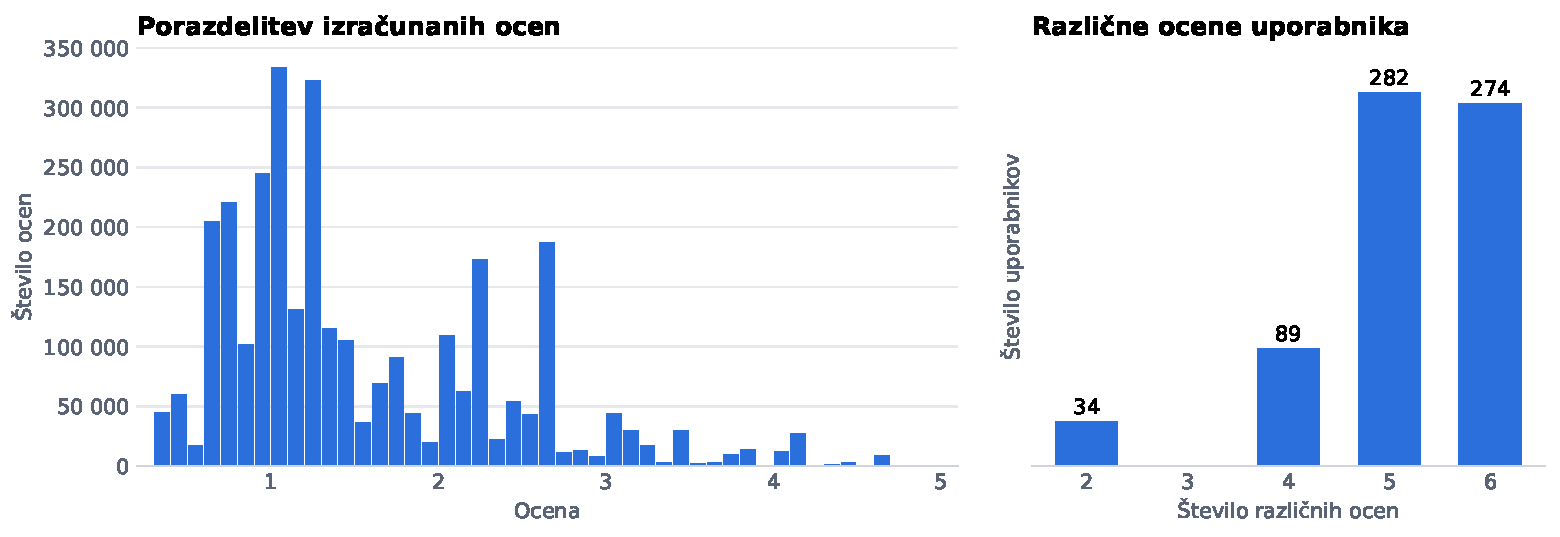
\includegraphics[width=\textwidth]{Slike/ratings_distribution.pdf}
\caption{Porazdelitev 3\,053\,029 izračunanih ocen (levo) in število
različnih ocen posameznega uporabnika (desno).}
\label{fig:ratings_hist}
\end{figure}

\subsection{Uporabniki}
\label{sec:data_users}
Izhodiščni vprašalniški podatki izvirajo iz raziskave
Inštituta Antona Trstenjaka za gerontologijo in
medgeneracijsko sožitje. Raziskava je obravnavala potrebe,
zmožnosti in stališča prebivalcev Slovenije, starih
50 let in več, podatki pa so bili zbrani z osebnimi
intervjuji. Izvorni nabor in njegova uporaba pri
modeliranju zdravega staranja sta opisana v delu
Gašperlin Stepančič in sodelavcev
\cite{gasperlin2024healthyageing}.

Izvorna raziskava je podrobneje predstavljena v
monografiji \emph{Staranje v Sloveniji}
\cite{ramovs2013staranje}, njen zdravstveni del
pa v analizi Voljča \cite{voljc2012zdravje}.

Vprašalniške odgovore je treba ločiti od ocen
priporočilnih elementov: odgovori izhajajo iz raziskave,
ocene kombinacij aktivnosti pa so v tem delu
izračunane s postopkom iz
razdelka~\ref{sec:data_rating_gen}.
Vhodna tabela ocen in uteži je vsebovala 696 uporabnikov
\cite{gasperlin2024healthyageing},
končni nabor, uporabljen v eksperimentih, pa 679.
Naknadno preverjanje vhodnih podatkov je pokazalo, da je
imelo vseh 17 uporabnikov, ki niso zastopani v končnem
naboru, pri vseh šestih uporabljenih vprašanjih o
aktivnostih odgovor 0. Pri teh uporabnikih niso manjkali
odgovori na uporabljena vprašanja ali vrednost uteži
\texttt{a\_F2}.

To je skladno z opisanim postopkom generiranja ocen:
pri ničelnih odgovorih so prispevki posameznih aktivnosti
enaki 0, ocena kombinacije pa ob kompatibilnostih na
intervalu $[0,1]$ ne preseže 0. Takšni zapisi zato ne
izpolnijo pogoja $r_{u,\mathbf{s}} > r_T$, kjer je
$r_T=0{,}3$.

\subsection{Aktivnosti}
\label{sec:data_activities}


Opisi aktivnosti in njihove kontekstne omejitve se berejo iz datoteke \texttt{ActivityContextGen\_v12.xlsx}. Za vsako aktivnost postopek uporabi:
\begin{itemize}
    \item vprašanje, s katerim je aktivnost povezana,
    \item časovni kontekst (npr. dopoldne, popoldne, kadarkoli),
    \item prostorski kontekst (npr. doma, v naravi, kjerkoli),
    \item pripadnost kontekstnim skupinam M3, M4 in M5.
\end{itemize}
Katalog vsebuje tudi druge, opisne lastnosti (npr. skupino aktivnosti in
povezavo z zdravstvenimi vidiki), ki jih postopek ne uporablja.

Katalog vključuje prehranske aktivnosti, telesno aktivnost in vsakodnevne opravke, na primer sestavo obroka in opravljanje poti peš.

Osnovni element priporočilnega modela ni nujno posamezna aktivnost,
temveč kombinacija od ene do treh aktivnosti. Kombinacijo označimo
z $i=(a_1,\ldots,a_m)$, kjer je $1 \leq m \leq 3$.
Vsaka različna kombinacija ima lasten identifikator in lastni vektor
latentnih faktorjev. Kombinacije z istim prvim članom zato niso
obravnavane kot isti element.

V posamezni kombinaciji se isti identifikator aktivnosti ne ponovi.
Zapis članov v terki je uporabljen za identifikacijo kombinacije
in ne določa časovnega vrstnega reda izvedbe. Sistem tako ne sestavlja
urnika aktivnosti.

Celotni katalog vsebuje 106 posameznih aktivnosti.
V uporabljenem eksperimentalnem naboru je zastopanih
34 posameznih aktivnosti, iz katerih je sestavljenih
6\,579 različnih kombinacij dolžine od ena do tri.
Število aktivnosti v katalogu zato ni enako številu
priporočilnih elementov, ki jih uporablja model.

Izbor aktivnosti je v uporabljeni konfiguraciji omejen
na vidik \texttt{activity}. Ta vključuje vprašanja
\texttt{Ac\_AB4\_1}, \texttt{Ac\_AB4\_2},
\texttt{Ac\_AB4\_3}, \texttt{Ac\_AB4\_4},
\texttt{Ac\_AB4\_5} in \texttt{Ac\_AB4\_8},
ki jim v katalogu pripada skupaj 34 aktivnosti.



\section{Algoritmi za priporočilne sisteme} 
\label{sec:recommender_algorithms}

Osnovne pristope priporočanja, vsebinsko in sodelovalno filtriranje ter
kontekstno zavedne sisteme, smo predstavili v
poglavju~\ref{sec:state_of_the_art}. Med modelno osnovanimi pristopi
sodelovalnega filtriranja je razširjena matrična faktorizacija, ki matriko
ocen predstavi z nizkorazsežnimi latentnimi faktorji uporabnikov in
elementov \cite{koren2009matrix}. Kontekst je mogoče upoštevati s
predfiltriranjem podatkov, z naknadnim filtriranjem priporočil ali
z neposrednim modeliranjem \cite{adomavicius2011context}.

\subsection{Izbira pristopa v tej nalogi}

V okviru te magistrske naloge smo uporabili modelno osnovan pristop sodelovalnega filtriranja z uporabo matrične faktorizacije (SVD) za napovedovanje izračunanih ocen kombinacij aktivnosti. Kontekstualne informacije niso vključene neposredno v fazi učenja modela, temveč se uporabijo v kasnejši fazi filtriranja priporočil. Takšna zasnova omogoča jasno ločitev med napovedovanjem izračunanih ocen in obravnavo konteksta ter poenostavlja eksperimentalno primerjavo med sistemom brez konteksta in sistemom s kontekstom.


\subsection{Pregled arhitekture sistema}
\label{sec:sys_architecture}

Na Sliki~\ref{fig:system_overview} je prikazan celoten potek delovanja
predlaganega priporočilnega sistema – od vhodnih podatkov, preko
generiranja ocen in učenja modela do končnih, kontekstualno filtriranih
priporočil. Arhitektura je zasnovana modularno, kar omogoča ločeno obravnavo
napovedovanja izračunanih ocen in obravnave kontekstualnih omejitev.

\begin{figure}[H]
\centering
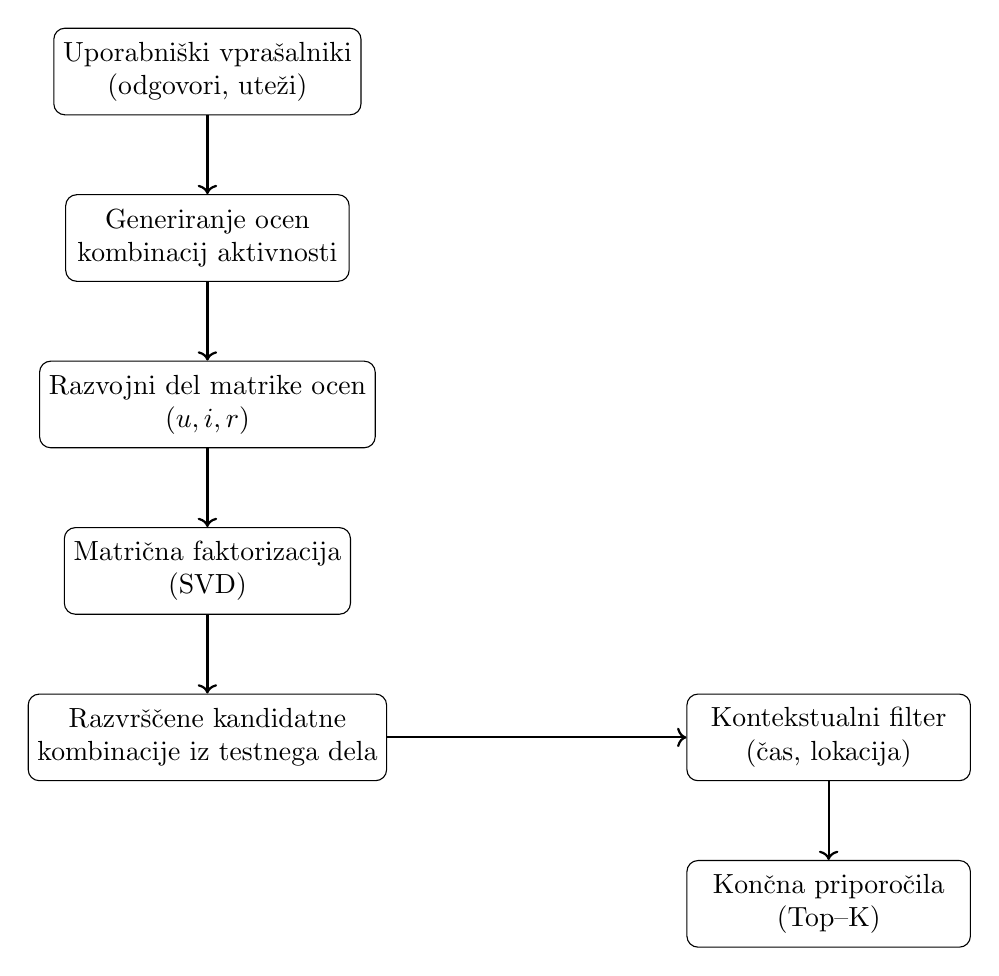
\begin{tikzpicture}[
    block/.style={
        rectangle, draw, rounded corners,
        align=center, minimum width=3.6cm, minimum height=1.1cm
    },
    arrow/.style={->, thick}
]


% Nodes
\node[block] (questionnaire) {Uporabniški vprašalniki\\(odgovori, uteži)};
\node[block, below=of questionnaire] (scoregen)
{Generiranje ocen\\kombinacij aktivnosti};
\node[block, below=of scoregen] (matrix)
{Razvojni del matrike ocen\\$(u,i,r)$};
\node[block, below=of matrix] (svd) {Matrična faktorizacija\\(SVD)};
\node[block, below=of svd] (topn)
{Razvrščene kandidatne\\kombinacije iz testnega dela};
\node[block, right=3.8cm of topn] (context) {Kontekstualni filter\\(čas, lokacija)};
\node[block, below=of context] (final) {Končna priporočila\\(Top--K)};

% Arrows
\draw[arrow] (questionnaire) -- (scoregen);
\draw[arrow] (scoregen) -- (matrix);
\draw[arrow] (matrix) -- (svd);
\draw[arrow] (svd) -- (topn);
\draw[arrow] (topn) -- (context);
\draw[arrow] (context) -- (final);

\end{tikzpicture}
\caption{Pregled postopka priporočanja kombinacij aktivnosti.
Model se uči na razvojnem delu podatkov, kandidatni seznam
pa se pri vrednotenju oblikuje iz odloženih testnih elementov.}
\label{fig:system_overview}
\end{figure}


\subsection{Generiranje ocen}
\label{sec:data_rating_gen}

V tem podrazdelku indeks $j$ označuje posamezno aktivnost,
$\mathbf{s}$ pa kombinacijo aktivnosti. V nadaljnjem opisu
priporočilnega modela je celotna kombinacija označena z $i$.

Ocene relevantnosti aktivnosti niso pridobljene z eksplicitnim ocenjevanjem
uporabnikov, temveč so izračunane na podlagi njihovih odgovorov na vprašalnik
in pripadajočih uporabniških uteži. Vsaka aktivnost $j$ je v katalogu povezana z vprašanjem
$q(j)$, katerega odgovor se uporabi pri izračunu njenega
prispevka. Odgovor ni nujno neposredno izražena
preferenca za aktivnost.

Naj bo $u$ uporabnik in $g$ izbrani vidik (npr. telesna aktivnost). Uporabniku
$u$ je za vsak vidik pripisana utež $s_u^{(g)}$, ki izraža splošno stopnjo
ustreznosti tega vidika. Poleg tega je na voljo surov odgovor uporabnika
$a_{u,q(j)}$ ter njegova min--max normalizirana vrednost $\tilde{a}_{u,q(j)} \in
[0,1]$.

Prispevek posamezne aktivnosti $j$ za uporabnika $u$ je definiran kot
\begin{equation}
r_{u,j}^{(1)} =
s_u^{(g)} \cdot a_{u,q(j)} \cdot \tilde{a}_{u,q(j)} .
\end{equation}

Vprašanje \texttt{Ac\_AB4\_8} označuje odsotnost
zavestne skrbi za zdravje. V uporabljeni izvedbi
pritrdilni odgovor poveča prispevek z njim povezanih
aktivnosti. Tega prispevka zato ne interpretiramo
kot neposredno izraženo uporabnikovo preferenco.
V sistemu so aktivnosti lahko združene tudi v krajše kombinacije
$\mathbf{s} = (j_1, j_2, \dots, j_m)$, kjer se skupna ocena kombinacije izračuna kot
vsota posameznih prispevkov:
\begin{equation}
R_u(\mathbf{s}) = \sum_{t=1}^{m} r_{u,j_t}^{(1)} .
\end{equation}

Za upoštevanje medsebojne skladnosti aktivnosti se uvede faktor kompatibilnosti
$C(\mathbf{s})$, definiran kot produkt parnih kompatibilnosti $\gamma_{j,\ell} \in
[0,1]$:
\begin{equation}
C(\mathbf{s}) =
\begin{cases}
1, & m = 1, \\
\prod_{1 \le p < q \le m} \gamma_{j_p,j_q}, & m > 1 .
\end{cases}
\end{equation}

Končna ocena kombinacije aktivnosti je nato definirana kot
\begin{equation}
r_{u,\mathbf{s}} = R_u(\mathbf{s}) - \left( 1 - C(\mathbf{s}) \right),
\end{equation}
kjer je $1 - C(\mathbf{s})$ kazen za nezdružljivost. Kompatibilnosti
so podane v listu \texttt{ActionCompatibilities} datoteke
\texttt{ActivityContextGen\_v12.xlsx}. V celotnem katalogu zavzamejo
vrednosti med 0 in 1, v uporabljenem bloku $34 \times 34$ pa samo 0 ali 1.
Zato je kazen enaka 0 ali natanko 1, ne glede na število nezdružljivih
parov v kombinaciji. Ker so uporabljeni odgovori dvojiški, je
$a_{u,q(j)} \cdot \tilde{a}_{u,q(j)} = a_{u,q(j)}$, ocena pred normalizacijo
pa je v praksi $s_u^{(g)}$ krat število pritrdilnih odgovorov v kombinaciji,
zmanjšano za 1, če kombinacija vsebuje nezdružljiv par.

V nadaljnjo obdelavo so vključene le aktivnosti oziroma kombinacije, za katere velja
$r_{u,\mathbf{s}} > r_T$, kjer je uporabljeni prag $r_T=0{,}3$. Preostale
ocene se nato linearno preslikajo na interval $[r_T, 5]$:
\begin{equation}
r'_{u,\mathbf{s}} =
r_T + (5 - r_T)\cdot
\frac{r_{u,\mathbf{s}} - r_{\min}}{r_{\max} - r_{\min}},
\end{equation}
kjer $r_{\min}$ in $r_{\max}$ predstavljata najmanjšo in največjo ohranjeno oceno pred normalizacijo.

Prag $r_T$ določa vključitev zapisa v generirani podatkovni nabor.
Ne predstavlja ločenega praga za določanje zadetkov pri vrednotenju
razvrščanja priporočil.

Generiranje in normalizacija ocen sta izvedena pred razdelitvijo
podatkov za učenje in vrednotenje. Eksperiment zato preverja
napovedovanje zadržanih ocen znotraj tako pripravljenega nabora;
referenčne ocene izhajajo iz istega postopka kot učne.


\subsection{Kontekstualne informacije in filtriranje}
\label{sec:rec_vs_act}

V podatkih razlikujemo dva tipa konteksta:
\begin{itemize}
    \item \textbf{REC kontekst} (\textit{recommendation context}): kontekst v trenutku, ko je priporočilo podano,
    \item \textbf{ACT kontekst} (\textit{action context}): kontekst v trenutku, ko je priporočena aktivnost dejansko izvedena.
\end{itemize}

Takšno upoštevanje konteksta je naknadno filtriranje
\cite{adomavicius2011context}. V obravnavanih eksperimentih uporabljamo oznake ACT, ki opisujejo
predvidene okoliščine izvedbe posamezne aktivnosti. Te oznake
predstavljajo lastnosti aktivnosti in niso meritve dejansko izvedenih
aktivnosti uporabnikov. Uporabljajo se pri neposrednem kontekstnem
filtriranju in pri obravnavi skupin aktivnosti s podobnimi
kontekstnimi opisi.

Za neposredno filtriranje vsakemu uporabniku določimo en simuliran
kontekst izvedbe $c=(C_T,C_P)$. Čas in kraj izberemo neodvisno
in enakomerno iz naborov različnih časovnih oziroma prostorskih
oznak v opisih ACT 34 priporočljivih aktivnosti
(11 časovnih in 9 prostorskih oznak). Izbrani kontekst velja za vse
kandidatne kombinacije tega uporabnika. Takšno vzorčenje ne
predstavlja empirične porazdelitve dejanskih uporabniških okoliščin.

Kombinacija je skladna s kontekstom le, če vsaka njena aktivnost
ustreza tako izbranemu času kot izbranemu kraju. To ne pomeni,
da se morajo aktivnosti izvajati hkrati. Oznaka \emph{kadarkoli}
pomeni odsotnost časovne omejitve, oznaka \emph{kjerkoli} pa
odsotnost prostorske omejitve. Obe pravili veljata tako za opis
aktivnosti kot za izbrani kontekst. Pri primerjavi oznak se odstranijo
začetni in končni presledki; druge oznake se primerjajo neposredno,
brez dodatnega sklepanja o njihovem pomenu.






\subsection{Končna struktura podatkov}
\label{sec:data_structure}

Končni podatkovni nabor je organiziran kot seznam zapisov oblike
\[
(u,i,\mathbf{c}_i,r'_{u,i}),
\]
kjer $u$ označuje uporabnika, $i$ kombinacijo aktivnosti,
$\mathbf{c}_i$ zbirko kontekstnih opisov njenih članov,
$r'_{u,i}$ pa izračunano in normalizirano oceno kombinacije.

Za učenje modela uporabimo triplete $(u,i,r'_{u,i})$.
Kontekstni opisi niso vhod v model SVD, temveč se uporabijo
pri naknadnem filtriranju kandidatnih priporočil. Simulirani
uporabnikov kontekst izvedbe se izbere posebej v fazi filtriranja.

\subsection{Definicija relevantnosti in izbor top-$N$/top-$K$ priporočil}
\label{sec:relevance_definition}

Pri vrednotenju razvrščanja za vsakega uporabnika obravnavamo
kombinacije aktivnosti, katerih ocene so v odloženem testnem delu.
Model te kombinacije razvrsti padajoče glede na napovedano oceno.
Začetni seznam vsebuje vse odložene testne kombinacije uporabnika.
Gre za razvrščanje zadržanih testnih elementov, ne za iskanje
po celotnem katalogu vseh možnih kombinacij.

V različici brez konteksta izberemo prvih največ $K=5$ kombinacij.
V različici s kontekstom vse odložene testne kombinacije uporabnika
filtriramo po pravilu skladnosti vseh članov kombinacije z izbranim
kontekstom in ohranimo prvih največ pet ustreznih kombinacij.
Če jih ustreza manj, vrnemo krajši seznam; seznam je lahko tudi prazen.

Pri različicah M3, M4 in M5 začetni seznam filtriramo ločeno
za vsako skupino. Kombinacija pripada skupini le, če tej skupini
pripadajo vse njene aktivnosti. Kombinacije s člani iz različnih
skupin so pri tem izločene. Uporabniku ne določimo ene ciljne
skupine, temveč priporočila in vrednotenje obravnavamo ločeno
po skupinah.

Za primerjavo uporabimo še razvrščanje po popularnosti, ki
testne kombinacije uporabnika razvrsti po povprečni oceni
kombinacije v razvojnem delu in vrne prvih pet, ter naključno
rangiranje, za katero izračunamo pričakovano vrednost metrik
(razdelek~\ref{sec:evaluation_metrics}). Obe primerjavi uporabita iste
kandidate, isti kontekstni filter in isto referenco kot SVD.

Referenčno množico za posameznega uporabnika sestavlja največ
pet kombinacij z najvišjimi izračunanimi ocenami v testnem delu
(globalna referenca). Različico z neposrednim kontekstnim
filtriranjem ovrednotimo z globalno in s kontekstno referenco.
Pri kontekstni referenci testne kombinacije pred izborom
filtriramo z istim kontekstom in pravilom skladnosti kot kandidate.
Pri M3, M4 in M5 referenčno
množico določimo znotraj posamezne skupine.

Zadetek pomeni ujemanje celotne priporočene kombinacije
z elementom referenčne množice. Ujemanje samo ene aktivnosti
v dveh različnih kombinacijah ne šteje kot zadetek.
Pri enakih referenčnih ocenah se vrstni red določi
leksikografsko po identifikatorjih aktivnosti v celotni
kombinaciji. Referenčna množica vsebuje največ pet
kombinacij in se pri strogi različici metrik ob izenačenih
ocenah ne razširi. Priporočena kombinacija zunaj te množice zato ne šteje
kot zadetek, tudi če ima enako referenčno oceno kot
peti izbrani element. Natančnost, priklic in F1-mera
tako merijo ujemanje z določeno referenčno množico,
na rezultat pa vpliva tudi pravilo razreševanja izenačenj.

Zato poročamo tudi F1-mero z izenačenji. Pri njej za relevantno
štejemo vsako kombinacijo, katere referenčna ocena je večja ali
enaka oceni petega referenčnega elementa (oziroma zadnjega,
če jih je manj kot pet).





\section{Matrična faktorizacija za priporočilni sistem} \label{sec:matrix_factorization}
Za napovedovanje ocen kombinacij aktivnosti uporabimo matrično
faktorizacijo. Model uporabnikom in kombinacijam priredi latentne
vektorje, iz katerih skupaj z odmiki izračuna napovedi ocen.

\subsection{Podatkovna matrika}

Vhod v model predstavlja matrika ocen $R$, katere vrstice ustrezajo
uporabnikom, stolpci pa različnim kombinacijam aktivnosti.
Element $r_{u,i}$ označuje normalizirano izračunano oceno
kombinacije $i$ za uporabnika $u$. V nadaljnjem opisu modela zaradi
preglednosti opustimo oznako za normalizacijo.

Matrika ni sestavljena iz neposrednih uporabniških ocen,
temveč iz ocen, pridobljenih s postopkom iz
razdelka~\ref{sec:data_rating_gen}. Model se uči samo iz zapisov
razvojnega dela podatkov; odložene testne ocene pri učenju
niso uporabljene.

\subsection{Model matrične faktorizacije}

Uporabimo model SVD iz knjižnice \textit{Surprise}
\cite{hug2020surprise}, ki izvaja matrično faktorizacijo z odmiki,
kot jo opisujejo Koren in sodelavca \cite{koren2009matrix}.
Model vsebuje matriko uporabniških latentnih faktorjev
$P \in \mathbb{R}^{|U|\times k}$ in matriko latentnih faktorjev
kombinacij aktivnosti $Q \in \mathbb{R}^{|I|\times k}$.
Množica $U$ vsebuje uporabnike, množica $I$ kombinacije aktivnosti,
$k$ pa označuje število latentnih dimenzij.

Napoved ocene kombinacije $i$ za uporabnika $u$ je
\[
\hat{r}_{u,i} = \mu + b_u + b_i + P_u^T Q_i,
\]
kjer je $\mu$ povprečje učnih ocen, $b_u$ odmik uporabnika,
$b_i$ odmik kombinacije, $P_u$ in $Q_i$ pa pripadajoča
latentna vektorja.

\paragraph{Interpretacija latentnih faktorjev.}
Vsak uporabnik ima svoj latentni vektor $P_u$, vsaka kombinacija
aktivnosti, zastopana v učnih podatkih, pa svoj latentni vektor $Q_i$.
Skalarni produkt $P_u^T Q_i$ predstavlja prispevek latentnega dela
k napovedani oceni. Posamezne latentne dimenzije nimajo vnaprej
določenega semantičnega pomena. Izpis teh vektorjev zato omogoča
vpogled v parametre modela, sam po sebi pa ne predstavlja
uporabniku razumljive razlage priporočila.


\subsection{Učenje modela}

Parametri modela se učijo z minimizacijo kvadratne napake med napovedanimi in referenčnimi izračunanimi ocenami ob uporabi regularizacije, ki omejuje velikost parametrov in zmanjšuje tveganje prenaučenosti. Optimizacija poteka z uporabo stohastičnega gradientnega spusta.

Hiperparametri modela so izbrani z mrežnim iskanjem na razvojnem
delu podatkov po postopku iz
razdelka~\ref{sec:experimental_protocol}.

\subsubsection{Hiperparametri modela SVD}
\label{sec:svd_hyperparams}

V knjižnici \textit{Surprise} je bil uporabljen model SVD z naslednjimi hiperparametri:
\begin{itemize}
    \item število latentnih faktorjev: $k=\texttt{n\_factors}$,
    \item število epoh učenja: $\texttt{n\_epochs}$,
    \item učna hitrost: $\gamma=\texttt{lr\_all}$,
    \item regularizacija: $\lambda=\texttt{reg\_all}$.
\end{itemize}

Končne vrednosti hiperparametrov so bile izbrane z mrežnim iskanjem (\textit{Grid Search}) na razvojnem delu podatkov, pri čemer je bil optimizacijski kriterij minimizacija RMSE. Izbrana konfiguracija je bila uporabljena pri dodatnem
preverjanju SVD na razvojnem delu ter pri končnem
vrednotenju vseh različic naknadnega filtriranja.


\subsection{Vloga matrične faktorizacije v sistemu}

Model SVD napoveduje izračunane ocene kombinacij aktivnosti,
ki niso bile vključene v učenje. Napovedi uporabimo za
razvrščanje kandidatnih kombinacij.

Referenčne ocene so določene s pravilom, ki združuje
vprašalniške odgovore, uporabniške uteži in združljivosti
aktivnosti. Napovedne metrike zato merijo približevanje
tem ocenam.

Časovni in prostorski kontekst upoštevamo pri naknadnem
filtriranju priporočil.


\section{Eksperimentalni protokol}
\label{sec:experimental_protocol}

Pred primerjavo algoritmov in izbiro hiperparametrov podatke
naključno razdelimo na razvojni del, ki vsebuje 75\,\% zapisov,
in odloženi testni del, ki vsebuje 25\,\% zapisov.
Razdelitev je izvedena na ravni zapisov uporabnik--kombinacija,
ne na ravni uporabnikov. Isti uporabnik je zato lahko zastopan
v obeh delih. Postopek ni namenjen vrednotenju priporočanja
za povsem nove uporabnike.

Na razvojnem delu primerjamo algoritme SVD, KNNBasic,
BaselineOnly in NMF. Uporabimo deset ponovitev metode
\texttt{ShuffleSplit}; v vsaki ponovitvi je 25\,\% razvojnih
zapisov namenjenih notranjemu preverjanju, preostali zapisi
pa učenju.

Za model SVD izvedemo mrežno iskanje hiperparametrov z
desetkratnim prečnim preverjanjem \texttt{KFold} na razvojnem delu.
Preizkusimo število latentnih faktorjev iz množice
$\{50,100,150\}$, število epoh iz $\{20,30\}$,
učno hitrost iz $\{0{,}002,0{,}005\}$ in regularizacijski
parameter iz $\{0{,}02,0{,}05\}$. Skupaj preizkusimo
24 konfiguracij. Kriterij izbire je najmanjša povprečna RMSE.

Izbrano konfiguracijo SVD dodatno ovrednotimo z desetimi
ponovitvami metode \texttt{ShuffleSplit} na razvojnem delu.
Ker je bil isti razvojni del uporabljen tudi za izbiro
hiperparametrov, teh rezultatov ne obravnavamo kot neodvisno
končno oceno uspešnosti.

Končni model naučimo na celotnem razvojnem delu in ga ovrednotimo
na odloženem testnem delu. Isti končni model in njegove testne
napovedi uporabimo pri vseh različicah naknadnega filtriranja.
Kontekstni filtri ne spreminjajo naučenih parametrov ali napovedanih
ocen, temveč samo izbor priporočenih kombinacij.

Za delitev podatkov in model SVD uporabimo naključno seme 42.
Končni rezultati temeljijo na polnem podatkovnem naboru.
Zagoni na prvih 100\,000 zapisih so namenjeni samo preverjanju
delovanja in niso uporabljeni za končne ugotovitve.


\section{Ovrednotenje uspešnosti priporočilnih sistemov} \label{sec:evaluation_metrics}
Za ovrednotenje kakovosti priporočilnih sistemov smo uporabili naslednje metrike:

\paragraph{RMSE (Root Mean Squared Error).} Meri kvadratni koren povprečne kvadratne napake med napovedanimi
in referenčnimi izračunanimi ocenami. Izračunana je kot:
\begin{equation}
\text{RMSE} = \sqrt{\frac{1}{n} \sum_{i=1}^n (\hat{r}_i - r_i)^2}
\label{eq:rmse}
\end{equation}

\paragraph{MAE (Mean Absolute Error).} Izračuna povprečno absolutno napako med ocenami:
\begin{equation}
\text{MAE} = \frac{1}{n} \sum_{i=1}^n |\hat{r}_i - r_i|
\label{eq:mae}
\end{equation}

\paragraph{MSE (Mean Squared Error).} Podobno kot RMSE, vendar brez kvadratnega korena:
\begin{equation}
\text{MSE} = \frac{1}{n} \sum_{i=1}^n (\hat{r}_i - r_i)^2
\label{eq:mse}
\end{equation}

\paragraph{FCP (Fraction of Concordant Pairs).} Metrika, ki meri delež parov, pri katerih sistem pravilno ohrani vrstni red med ocenami.

\paragraph{Čas učenja.} Povprečen čas trajanja učenja modela na posameznem razdelku podatkov, izražen v sekundah.

\paragraph{Natančnost, priklic in F1-mera.}
Naj bo $A_u$ neprazna referenčna množica največ petih kombinacij
za uporabnika $u$, $B_u$ pa množica dejansko vrnjenih
priporočil, ki prav tako vsebuje največ pet kombinacij.
Natančnost in priklic izračunamo kot
\[
\mathrm{Prec}_u =
\begin{cases}
\dfrac{|A_u \cap B_u|}{|B_u|}, & |B_u|>0,\\
0, & |B_u|=0,
\end{cases}
\qquad
\mathrm{Rec}_u = \frac{|A_u \cap B_u|}{|A_u|}.
\]
F1-mera je
\[
F1_u =
\begin{cases}
\dfrac{2\,\mathrm{Prec}_u\,\mathrm{Rec}_u}
{\mathrm{Prec}_u+\mathrm{Rec}_u}, & \mathrm{Prec}_u+\mathrm{Rec}_u>0,\\
0, & \mathrm{Prec}_u+\mathrm{Rec}_u=0.
\end{cases}
\]

Metrike izračunamo za uporabnike z neprazno referenčno množico
in nato za vsako metriko posebej izračunamo aritmetično
povprečje po uporabnikih. Uporabniki brez vrnjenih priporočil
ostanejo vključeni z vrednostmi nič.
Povprečna F1-mera je povprečje uporabniških F1-mer, ne
harmonična sredina že povprečenih natančnosti in priklica.
Imenovalec natančnosti je dejansko število vrnjenih priporočil,
ki je lahko manjše od pet.

\paragraph{F1-mera z izenačenji.}
Naj bo $\rho_u$ najnižja referenčna ocena v množici $A_u$ in $A'_u$
množica vseh kombinacij, iz katerih je bila izbrana $A_u$,
z oceno vsaj $\rho_u$. F1-mero z izenačenji (v tabeli F1 z izen.) izračunamo enako
kot F1-mero, pri čemer število zadetkov $|A_u\cap B_u|$ nadomestimo
z $|A'_u\cap B_u|$, imenovalec priklica pa ostane $|A_u|$.

\paragraph{Pokritost.}
Pokritost je delež vseh testnih uporabnikov, ki so prejeli
vsaj eno priporočilo.

Pri kontekstni referenci uporabnik brez skladnih testnih
kombinacij nima referenčne množice in ni vključen v povprečje.

Pri M3, M4 in M5 se referenčne množice določijo ločeno po
skupinah. Uporabnik brez referenčnih elementov v posamezni
skupini ni vključen v njeno povprečje. Če skupina nima
nobenega uporabnika z referenčnimi elementi, implementacija
zanjo vrne ničelne metrike. Skupni rezultat posamezne
segmentacije je povprečje rezultatov njenih skupin, uteženo
s številom uporabnikov z neprazno referenčno množico v skupini.

Segmentirane različice in kontekstna referenca imajo drugačne referenčne množice
in lahko drugačne množice uporabnikov, zato njihovih vrednosti
ne primerjamo neposredno z različico brez konteksta.

\paragraph{Pričakovana vrednost naključnega rangiranja.}
Naj ima uporabnik $n_u$ kandidatov. Naključno urejen seznam vrne
$b_u=\min(5,n_u)$ kombinacij. Če je med kandidati $h_u$ elementov
referenčne množice $A_u$, je pričakovano število zadetkov
$b_u h_u/n_u$. F1-mero lahko zapišemo kot
$2|A_u\cap B_u|/(|A_u|+|B_u|)$, zato je
\begin{equation}
\mathrm{E}[F1_u] = \frac{2\,b_u\,h_u}{n_u\,(|A_u|+b_u)} .
\label{eq:random_f1}
\end{equation}
Pri kontekstni referenci so kandidati hkrati osnova za referenco
in velja $|A_u|=b_u=h_u=\min(5,n_u)$, zato je
$\mathrm{E}[F1_u]=\min(5,n_u)/n_u$. Pri F1-meri z izenačenji $h_u$
nadomestimo s številom kandidatov v množici $A'_u$. Vrednosti so
izračunane analitično, brez naključnega vzorčenja.

\paragraph{Povprečna referenčna ocena.}
Za vrnjena priporočila poročamo povprečje njihovih izračunanih
ocen v testnem delu (v tabeli Povp.\ ref.\ ocena). Pri segmentiranih
različicah je povprečje izračunano čez vsa vrnjena priporočila
vseh skupin, pri naključnem rangiranju pa je to pričakovana vrednost.

RMSE, MAE, MSE in FCP smo izračunali s funkcijami iz knjižnice \texttt{Surprise}, metrike razvrščanja pa z lastnimi Python funkcijami.

\section{Python knjižnice} \label{sec:python_libraries}

Razvoj in evalvacija priporočilnega sistema sta bila izvedena v programskem jeziku Python. V nadaljevanju so na kratko opisane ključne knjižnice, ki so bile uporabljene pri implementaciji sistema, obdelavi podatkov in eksperimentalni analizi.

\paragraph{NumPy.}
Knjižnica \texttt{NumPy} je bila uporabljena za numerične operacije, delo z vektorji in matrikami ter za učinkovito izvajanje matematičnih izračunov, povezanih z uteževanjem ocen in matrično faktorizacijo.

\paragraph{Pandas.}
Knjižnica \texttt{pandas} je bila uporabljena za obdelavo in analizo podatkov, branje vhodnih podatkov iz datotek formata \texttt{.xlsx} ter za organizacijo eksperimentalnih rezultatov v tabelarični obliki. Poleg tega je bila uporabljena za shranjevanje rezultatov evalvacije v datoteke formata \texttt{.xlsx} in \texttt{.tex}.

\paragraph{Scikit-learn.}
Iz knjižnice \texttt{scikit-learn} sta uporabljena razreda \texttt{ShuffleSplit} (delitev na razvojni in odloženi testni del) in \texttt{MinMaxScaler} (normalizacija odgovorov).

\paragraph{Surprise.}
Knjižnica \texttt{Surprise} je predstavljala osrednje ogrodje za implementacijo priporočilnega sistema. Uporabljena je bila za primerjane algoritme (SVD, KNNBasic, BaselineOnly in NMF), prečno preverjanje in mrežno iskanje, napovedovanje ocen ter izračun metrik RMSE, MAE, MSE in FCP.

\paragraph{Matplotlib.}
Knjižnica \texttt{matplotlib} je bila uporabljena za izris grafov.

\paragraph{Druge knjižnice.}
Poleg navedenih knjižnic so bile uporabljene tudi standardne Python knjižnice, kot so \texttt{pickle} za shranjevanje in nalaganje vmesnih podatkovnih struktur, \texttt{time} za merjenje časovne zahtevnosti algoritmov ter \texttt{pathlib} za delo z datotečnim sistemom in upravljanje poti do datotek. Knjižnica \texttt{SciPy} je uporabljena samo posredno, kot odvisnost drugih knjižnic.



\chapter{Eksperimentalni rezultati} \label{chap:results}
V tem poglavju so predstavljeni eksperimentalni rezultati evalvacije priporo\-čilnega sistema. Najprej analiziramo uspešnost osnovnega sistema brez upoštevanja kontekstualnih informacij, ki služi kot referenčno izhodišče. Nato predstavimo rezultate sistema, pri katerem so kontekstualne informacije vključene z naknadnim filtriranjem priporočil. V nadaljevanju obravnavamo še razširjeni primer z uporabo grupiranih kontekstov. Rezultati so predstavljeni s standardnimi metrikami za napovedovanje ocen ter z metrikami za ocenjevanje kakovosti razvrščanja priporočil, pri čemer je poudarek na primerjalni analizi vpliva konteksta na delovanje sistema.


\section{Uspešnost priporočilnega sistema brez konteksta} \label{sec:results_without_context}
Za oceno osnovne uspešnosti priporočilnega sistema brez upoštevanja kontekstualnih informacij smo uporabili algoritem SVD (Singular Value Decomposition), implementiran v knjižnici \textit{Surprise}. Podatkovna matrika je bila generirana na podlagi ocen aktivnosti, ki izhajajo iz uporabniških odgovorov in pripadajočih uteži, brez vključevanja časovnega ali prostorskega konteksta.


\paragraph{Konfiguracija eksperimenta.}
Eksperiment sledi protokolu iz
razdelka~\ref{sec:experimental_protocol}. Primerjava algoritmov
in izbira hiperparametrov potekata na razvojnem delu podatkov.
Končni model je naučen na celotnem razvojnem delu in ovrednoten
na odloženem testnem delu.



Mrežno iskanje na razvojnem delu je izbralo konfiguracijo SVD
s 150 latentnimi faktorji, 30 epohami, učno hitrostjo
$0{,}005$ in regularizacijskim parametrom $0{,}02$.
Najnižja povprečna RMSE v mrežnem iskanju je znašala
$0{,}08444$. Vse štiri izbrane vrednosti so na robu preizkušene
mreže, zato je optimum lahko zunaj nje.



\paragraph{Ocenjevalne metrike.} 
Uspešnost sistema smo ovrednotili z uporabo metrik RMSE (Root Mean Squared Error), MAE (Mean Absolute Error), FCP (Fraction of Concordant Pairs) in MSE (Mean Squared Error), ki so primerne za ocenjevanje natančnosti napovedovanja ocen in so opisane v poglavju~\ref{sec:evaluation_metrics}. 



\paragraph{Rezultati.} 
Tabela~\ref{tab:cv_results_tuned_svd} prikazuje povprečne rezultate
desetih ponovitev preverjanja izbrane konfiguracije SVD na
razvojnem delu. Ker je bil ta del uporabljen tudi za izbiro
hiperparametrov, tabela ne predstavlja končnega vrednotenja
na odloženem testnem delu.

% Prva izvedba ShuffleSplit
\begin{table}[htbp]
\centering
\caption{Rezultati izbrane konfiguracije SVD na razvojnem delu:
deset ponovitev metode ShuffleSplit.}
\label{tab:cv_results_tuned_svd}
\begin{tabular}{lrr}
\toprule
Metrika & Povprečje & Standardni odklon \\
\midrule
RMSE & 0,089465 & 0,000418 \\
MAE & 0,056712 & 0,000152 \\
MSE & 0,008004 & 0,000075 \\
FCP & 0,995945 & 0,000148 \\
Čas učenja [s] & 42,650 & 0,989 \\
Čas napovedovanja [s] & 3,261 & 0,774 \\
\bottomrule
\end{tabular}
\end{table}


Za lažjo primerjavo uspešnosti posameznih priporočilnih algoritmov so
povprečne vrednosti napake RMSE prikazane tudi grafično na
Sliki~\ref{fig:algo_rmse_comparison}.

Na razvojnem delu smo primerjali algoritme SVD, KNNBasic,
BaselineOnly in NMF z metodo \texttt{ShuffleSplit}.
Rezultati so prikazani v Tabeli~\ref{tab:algorithm_comparison}.
SVD je uporabljen kot osnovni model za nadaljnjo obravnavo
naknadnega filtriranja; primerjava algoritmov omogoča presojo
njegove napovedne uspešnosti glede na druge obravnavane pristope.

\begin{table}[htbp]
\centering
\caption{Primerjava algoritmov na razvojnem delu podatkov (ShuffleSplit, 10 ponovitev, 25\% test).}
\label{tab:algorithm_comparison}
\begin{tabular}{lrrrr}
\toprule
Algoritem & RMSE & MAE & MSE & FCP \\
\midrule
SVD & 0,105 & 0,065 & 0,011 & 0,994 \\
KNNBasic & 0,297 & 0,158 & 0,088 & 0,949 \\
BaselineOnly & 0,473 & 0,366 & 0,224 & 0,878 \\
NMF & 0,270 & 0,180 & 0,073 & 0,959 \\
\bottomrule
\end{tabular}

\end{table}


Med primerjanimi algoritmi je SVD na razvojnem delu dosegel
najnižjo povprečno RMSE, in sicer $0{,}1047$.
Sledili so NMF z $0{,}2700$, KNNBasic z $0{,}2974$
in BaselineOnly z $0{,}4734$.
Primerjava se nanaša na konfiguracije algoritmov, uporabljene
v tem poskusu; mrežno iskanje hiperparametrov je bilo nato
izvedeno samo za SVD.

\begin{figure}[H]
\centering
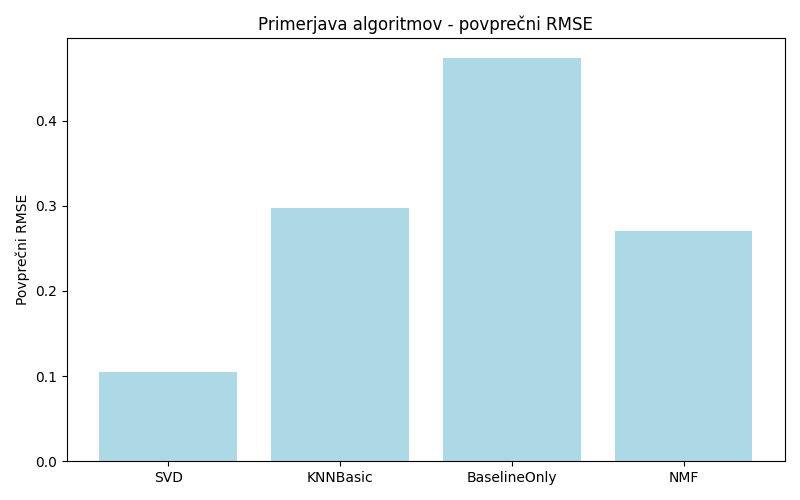
\includegraphics[width=0.75\textwidth]{Slike/algorithm_rmse_comparison_20261015_150006.png}
\caption{Primerjava povprečne vrednosti RMSE za različne priporočilne algoritme.}
\label{fig:algo_rmse_comparison}
\end{figure}

\paragraph{Končno vrednotenje na odloženem testnem delu.}
Končni model SVD je bil naučen na 2\,289\,771 razvojnih
ocenah in ovrednoten na 763\,258 odloženih testnih ocenah.
Rezultati so prikazani v Tabeli~\ref{tab:heldout_svd}.
Primerjava algoritmov in izbira hiperparametrov sta iz zagona
15.~10.~2026, vrednotenje priporočil pa iz zagona 25.~11.~2026,
v katerem je bil isti model ponovno naučen in je dosegel
enake testne metrike.

\begin{table}[htbp]
\centering
\caption{Uspešnost končnega modela SVD na odloženem testnem delu.}
\label{tab:heldout_svd}
\begin{tabular}{lr}
\toprule
Metrika & Vrednost \\
\midrule
RMSE & 0,0819 \\
MAE & 0,0531 \\
MSE & 0,0067 \\
FCP & 0,9966 \\
\bottomrule
\end{tabular}
\end{table}

Nizki vrednosti RMSE in MAE kažeta majhno odstopanje
napovedi od izračunanih referenčnih ocen v obravnavanem
naboru. Visoka vrednost FCP kaže dobro ohranjanje
vrstnega reda pri primerjavah parov ocen.
To ne pomeni nujno enake uspešnosti pri izboru nekaj
najvišje ocenjenih kombinacij, kar preverimo ločeno
z metrikami razvrščanja.

\paragraph{Izbor petih kombinacij.}
Ujemanje izbranih kombinacij z referenčno množico
ocenimo z natančnostjo, priklicem in F1-mero. Referenčne množice in izbor priporočil
so določeni v razdelku~\ref{sec:relevance_definition},
izračun metrik pa v razdelku~\ref{sec:evaluation_metrics}.
Rezultati vseh različic so zbrani v
Tabeli~\ref{tab:results_all_layers} in na
Sliki~\ref{fig:rezultati_metrike}. Natančnost in priklic sta pri vseh
različicah enaka F1-meri, zato navajamo le slednjo. Pri različici brez
konteksta enakost izhaja iz tega, da imata priporočena in referenčna
množica za vsakega uporabnika po pet elementov.

Različica brez konteksta je vrnila 3\,395 priporočil,
to je pet kombinacij za vsakega od 679 uporabnikov (pokritost $1{,}000$).
F1-mera znaša $0{,}339$, F1-mera z izenačenji $0{,}982$, povprečna
referenčna ocena vrnjenih kombinacij pa $3{,}066$. Razvrščanje po
popularnosti doseže F1-mero $0{,}151$, z izenačenji $0{,}531$, pri
povprečni referenčni oceni $2{,}882$. Pričakovane vrednosti naključnega
rangiranja so $0{,}006$, $0{,}066$ in $1{,}468$.

Naknadno preverjanje je pokazalo izenačenje referenčnih
ocen na meji top-5 pri 658 od 679 uporabnikov
(96,9~\%). Med 2\,244 priporočili osnovne različice,
ki niso pripadala izbrani referenčni množici, jih je
imelo 2\,184 (97,3~\%) natanko enako referenčno oceno
kot peti element te množice. Večina teh nezadetkov
zato ne pomeni nižje referenčne ocene, temveč izbiro
druge kombinacije med enako ocenjenimi možnostmi.
F1-mero $0{,}339$ zato razlagamo skupaj z F1-mero z izenačenji:
prva meri ujemanje z določeno referenčno množico ob uporabljenem
pravilu razreševanja izenačenj, druga pa ne razlikuje med enako
ocenjenimi kombinacijami. Omejitve te razlage so zbrane v
razdelku~\ref{sec:limitations}.

Model, ki bi vse testne ocene napovedal brez napake in izenačenja
razreševal naključno, bi dosegel pričakovano strogo F1-mero $0{,}321$.
Vrednost $0{,}339$ je torej na ravni, ki jo stroga mera ob izenačenjih
dopušča tudi brezhibnemu napovedovanju ocen; razlika do 1 izhaja predvsem
iz razreševanja izenačenj in ne iz napak napovedi.


\section{Uspešnost priporočilnega sistema s kontekstom} 
\label{sec:results_with_context}

V tem eksperimentu uporabimo isti končni model SVD kot pri
različici brez konteksta. Kontekst vključimo z naknadnim
filtriranjem kandidatnih kombinacij.

\paragraph{Uporabljen kontekst.}
Vsakemu uporabniku določimo en simuliran časovni in prostorski
kontekst izvedbe na podlagi oznak ACT. Postopek izbire konteksta
in pravilo skladnosti vseh aktivnosti v kombinaciji sta opisana
v razdelku~\ref{sec:rec_vs_act}.

\paragraph{Konfiguracija eksperimenta.}
Obe različici uporabljata iste odložene testne podatke in
kot kandidate vse odložene testne kombinacije uporabnika.
Različica s kontekstom izbere največ pet kombinacij, ki prestanejo
filter. Ta ne spremeni napovedanih ocen ali medsebojnega vrstnega
reda ohranjenih kandidatov.

\paragraph{Ocenjevalne metrike.}
Uporabimo natančnost, priklic in F1-mero z globalno referenco,
enako kot pri različici brez konteksta, in s kontekstno referenco.
Dodatno poročamo F1-mero z izenačenji, pokritost in
povprečno referenčno oceno vrnjenih priporočil.

\paragraph{Rezultati.}
Rezultati z globalno in s kontekstno referenco so v
Tabeli~\ref{tab:results_all_layers}, razčlenitev uporabnikov pa v
Tabeli~\ref{tab:context_breakdown}.

Kontekstna različica je vrnila 2\,534 priporočil za 608
od 679 uporabnikov (pokritost $0{,}895$).
Preostalih 71 uporabnikov ni prejelo nobenega priporočila,
ker nobena od njihovih odloženih testnih kombinacij
ni prestala kontekstnega filtra. Od teh jih ima 23 skladno kombinacijo
v razvojnem delu, torej jih brez priporočila pusti delitev podatkov;
pri 48 skladne kombinacije ni v celotnem naboru, torej je razlog
kontekstni filter.

Z globalno referenco znaša F1-mera $0{,}018$, z izenačenji
$0{,}120$. V to povprečje so vključeni tudi uporabniki
brez priporočil, pri katerih so metrike enake nič.
Vrednost je nizka, ker vrnjene kombinacije primerjamo s kombinacijami,
ki niso izbrane glede na kontekst; pričakovana vrednost naključnega
rangiranja istih skladnih kandidatov je $0{,}001$.

S kontekstno referenco znaša F1-mera $0{,}804$, z izenačenji
$0{,}998$; upoštevanih je 608 uporabnikov z neprazno
referenco. Povprečna referenčna ocena vrnjenih priporočil
je $2{,}045$, pri popularnosti $1{,}942$ in pri naključnem
rangiranju $1{,}425$.

\begin{table}[htbp]
\centering
\caption{F1 s kontekstno referenco glede na število skladnih testnih kombinacij uporabnika. Naključno je pričakovana vrednost naključnega rangiranja skladnih kombinacij.}
\label{tab:context_breakdown}
\footnotesize
\setlength{\tabcolsep}{4pt}
\begin{tabular}{lrrrr}
\toprule
Skladne testne kombinacije & Uporabniki & SVD & Popularnost & Naključno \\
\midrule
0 (skladna le v razvojnem delu) & 23 & -- & -- & -- \\
0 (brez skladne v celotnem naboru) & 48 & -- & -- & -- \\
1–5 & 210 & 1,000 & 1,000 & 1,000 \\
več kot 5 & 398 & 0,700 & 0,569 & 0,285 \\
skupaj vsaj 1 & 608 & 0,804 & 0,718 & 0,532 \\
\bottomrule
\end{tabular}

\end{table}


\paragraph{Primerjava z naključnim rangiranjem in popularnostjo.}
Del visoke vrednosti je posledica majhnega števila kandidatov:
pri 210 od 679 uporabnikov (30,9~\%) je skladnih največ pet
testnih kombinacij (in vsaj ena), zato so vse hkrati priporočene
in referenčne, F1-mera pa je 1 pri vsakem razvrščanju. Informativna
je primerjava na 398 uporabnikih z več kot petimi skladnimi
kombinacijami: naključno rangiranje doseže $0{,}285$, popularnost
$0{,}569$ in SVD $0{,}700$, z izenačenji pa $0{,}470$, $0{,}857$
in $0{,}996$. Na vseh 608 uporabnikih so vrednosti
$0{,}532$, $0{,}718$ in $0{,}804$.

\paragraph{Primera priporočil.}
Pri simuliranem kontekstu \emph{ob kosilu, v naselju} je bila
enemu od uporabnikov priporočena kombinacija »Obrok naj bo bogat
z beljakovinami.« in »Danes dnevne opravke v čimvečji meri opravite
peš.« Prva aktivnost ima oznaki \emph{ob kosilu} in \emph{kjerkoli},
druga \emph{kadarkoli} in \emph{kjerkoli}, zato obe ustrezata kontekstu.
Aktivnosti sta združljivi. Napovedana ocena je $3{,}372$,
referenčna pa $3{,}392$.

Primer vsebinsko slabega priporočila je kombinacija, izbrana pri kontekstu
\emph{ob kosilu, v naravi}: »V obrok vključite zelenjavo.«,
»Obrok naj bo bogat z beljakovinami.« in še enkrat »Obrok naj bo bogat
z beljakovinami.« Zadnji dve aktivnosti imata isto besedilo, a
različna identifikatorja (vprašanji \texttt{Ac\_AB4\_1} in
\texttt{Ac\_AB4\_8}). Vsi trije pari so v matriki združljivosti
označeni kot nezdružljivi, kazen pa je kljub temu samo 1. Napovedana
ocena je $2{,}676$, referenčna $2{,}634$. Pogostost takšnih
kombinacij obravnava razdelek~\ref{sec:limitations}.


\section{Uspešnost priporočilnega sistema z grupiranimi konteksti} 
\label{sec:grouped_contexts}
V tem razdelku obravnavamo različice M3, M4 in M5,
ki aktivnosti razdelijo v tri, štiri oziroma pet skupin
glede na njihove kontekstne opise ACT.
Oznake opisujejo predvidene okoliščine izvedbe aktivnosti,
ne opazovanega vedenja uporabnikov.

Pri priporočanju se za vsako skupino ohranijo samo kombinacije,
katerih vse aktivnosti pripadajo tej skupini. Priporočila
in referenčne množice se vrednotijo ločeno po skupinah.


\subsection{Nenadzorovano razvrščanje kontekstov v skupine}

Pri priporočanju uporabljamo vnaprej določene
pripadnosti aktivnosti skupinam, zapisane v stolpcih
\texttt{ContextG\_act\_3},
\texttt{ContextG\_act\_4} in
\texttt{ContextG\_act\_5} datoteke
\texttt{ActivityContextGen\_v12.xlsx}.
V končnem eksperimentu teh pripadnosti ne
izračunavamo ponovno, temveč jih uporabimo
pri filtriranju kombinacij aktivnosti.

Na Sliki~\ref{fig:elbow_actC} je prikazana komolčna krivulja, ki prikazuje odvisnost inercije od števila segmentov $k$.

\begin{figure}[H]
    \centering
    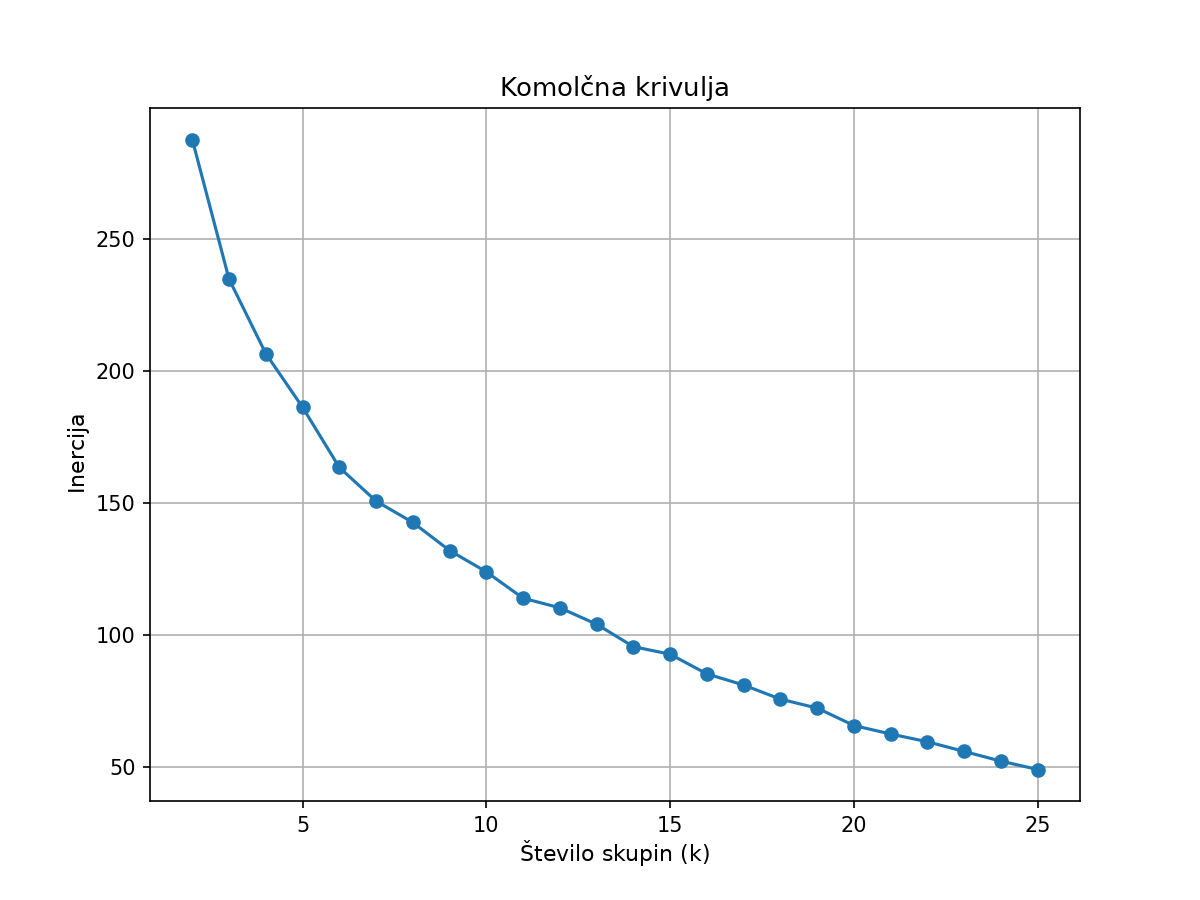
\includegraphics[width=0.75\linewidth]{Slike/ContextGroup_inertia_actC.png}
    \caption{Komolčna krivulja za presojo števila skupin na podlagi opisov ACT. Vir: analiza mentorja prof.~dr.~Andreja Koširja; koda ni del repozitorija.}
    \label{fig:elbow_actC}
\end{figure}

Inercija se z večanjem števila skupin zmanjšuje.
Krivulja ne določa enoznačnega optimalnega
števila skupin. V nadaljevanju obravnavamo tri
razpoložljive razdelitve aktivnosti:

\begin{itemize}
    \item M3 -- segmentacija v 3 skupine,
    \item M4 -- segmentacija v 4 skupine,
    \item M5 -- segmentacija v 5 skupin.
\end{itemize}

Na Sliki~\ref{fig:dendrogram_actC} je prikazan dendrogram hierarhičnega združevanja.

\begin{figure}[H]
    \centering
    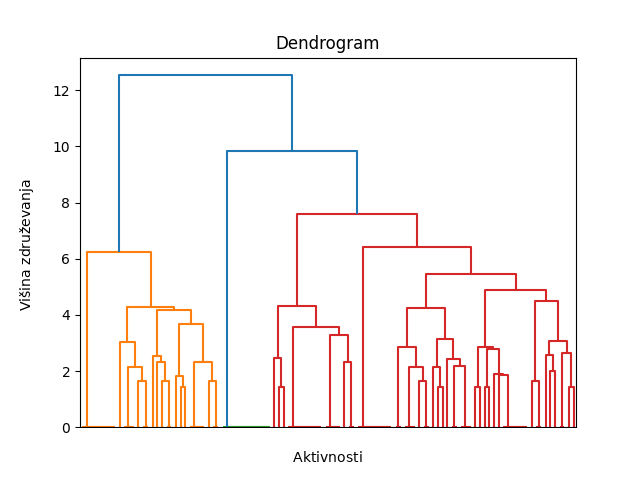
\includegraphics[width=0.9\linewidth]{Slike/ContextGroup_dendrogram_agg_actC.png}
    \caption{Dendrogram hierarhičnega razvrščanja opisov ACT v skupine. Vir: analiza mentorja prof.~dr.~Andreja Koširja; koda ni del repozitorija.}
    \label{fig:dendrogram_actC}
\end{figure}

Dendrogram prikazuje hierarhične podobnosti med kontekstnimi
opisi. Razdelitve M3, M4 in M5 niso njegovi rezi: gre za tri
ločene razdelitve, ki niso gnezdene. Skupine so fiksen vhod iz
datoteke Excel, koda za njihov izračun pa ni del repozitorija.

\subsection{Porazdelitev kontekstnih oznak v katalogu}

Slika~\ref{fig:hists_actC} prikazuje pogostost časovnih
in prostorskih oznak ACT v celotnem katalogu
106 aktivnosti. Posamezna aktivnost ima lahko več
časovnih in prostorskih oznak, zato vsota njihovih
pogostosti lahko presega število aktivnosti.
Vsaka oznaka je pri posamezni aktivnosti šteta
največ enkrat.

\begin{figure}[H]
    \centering
    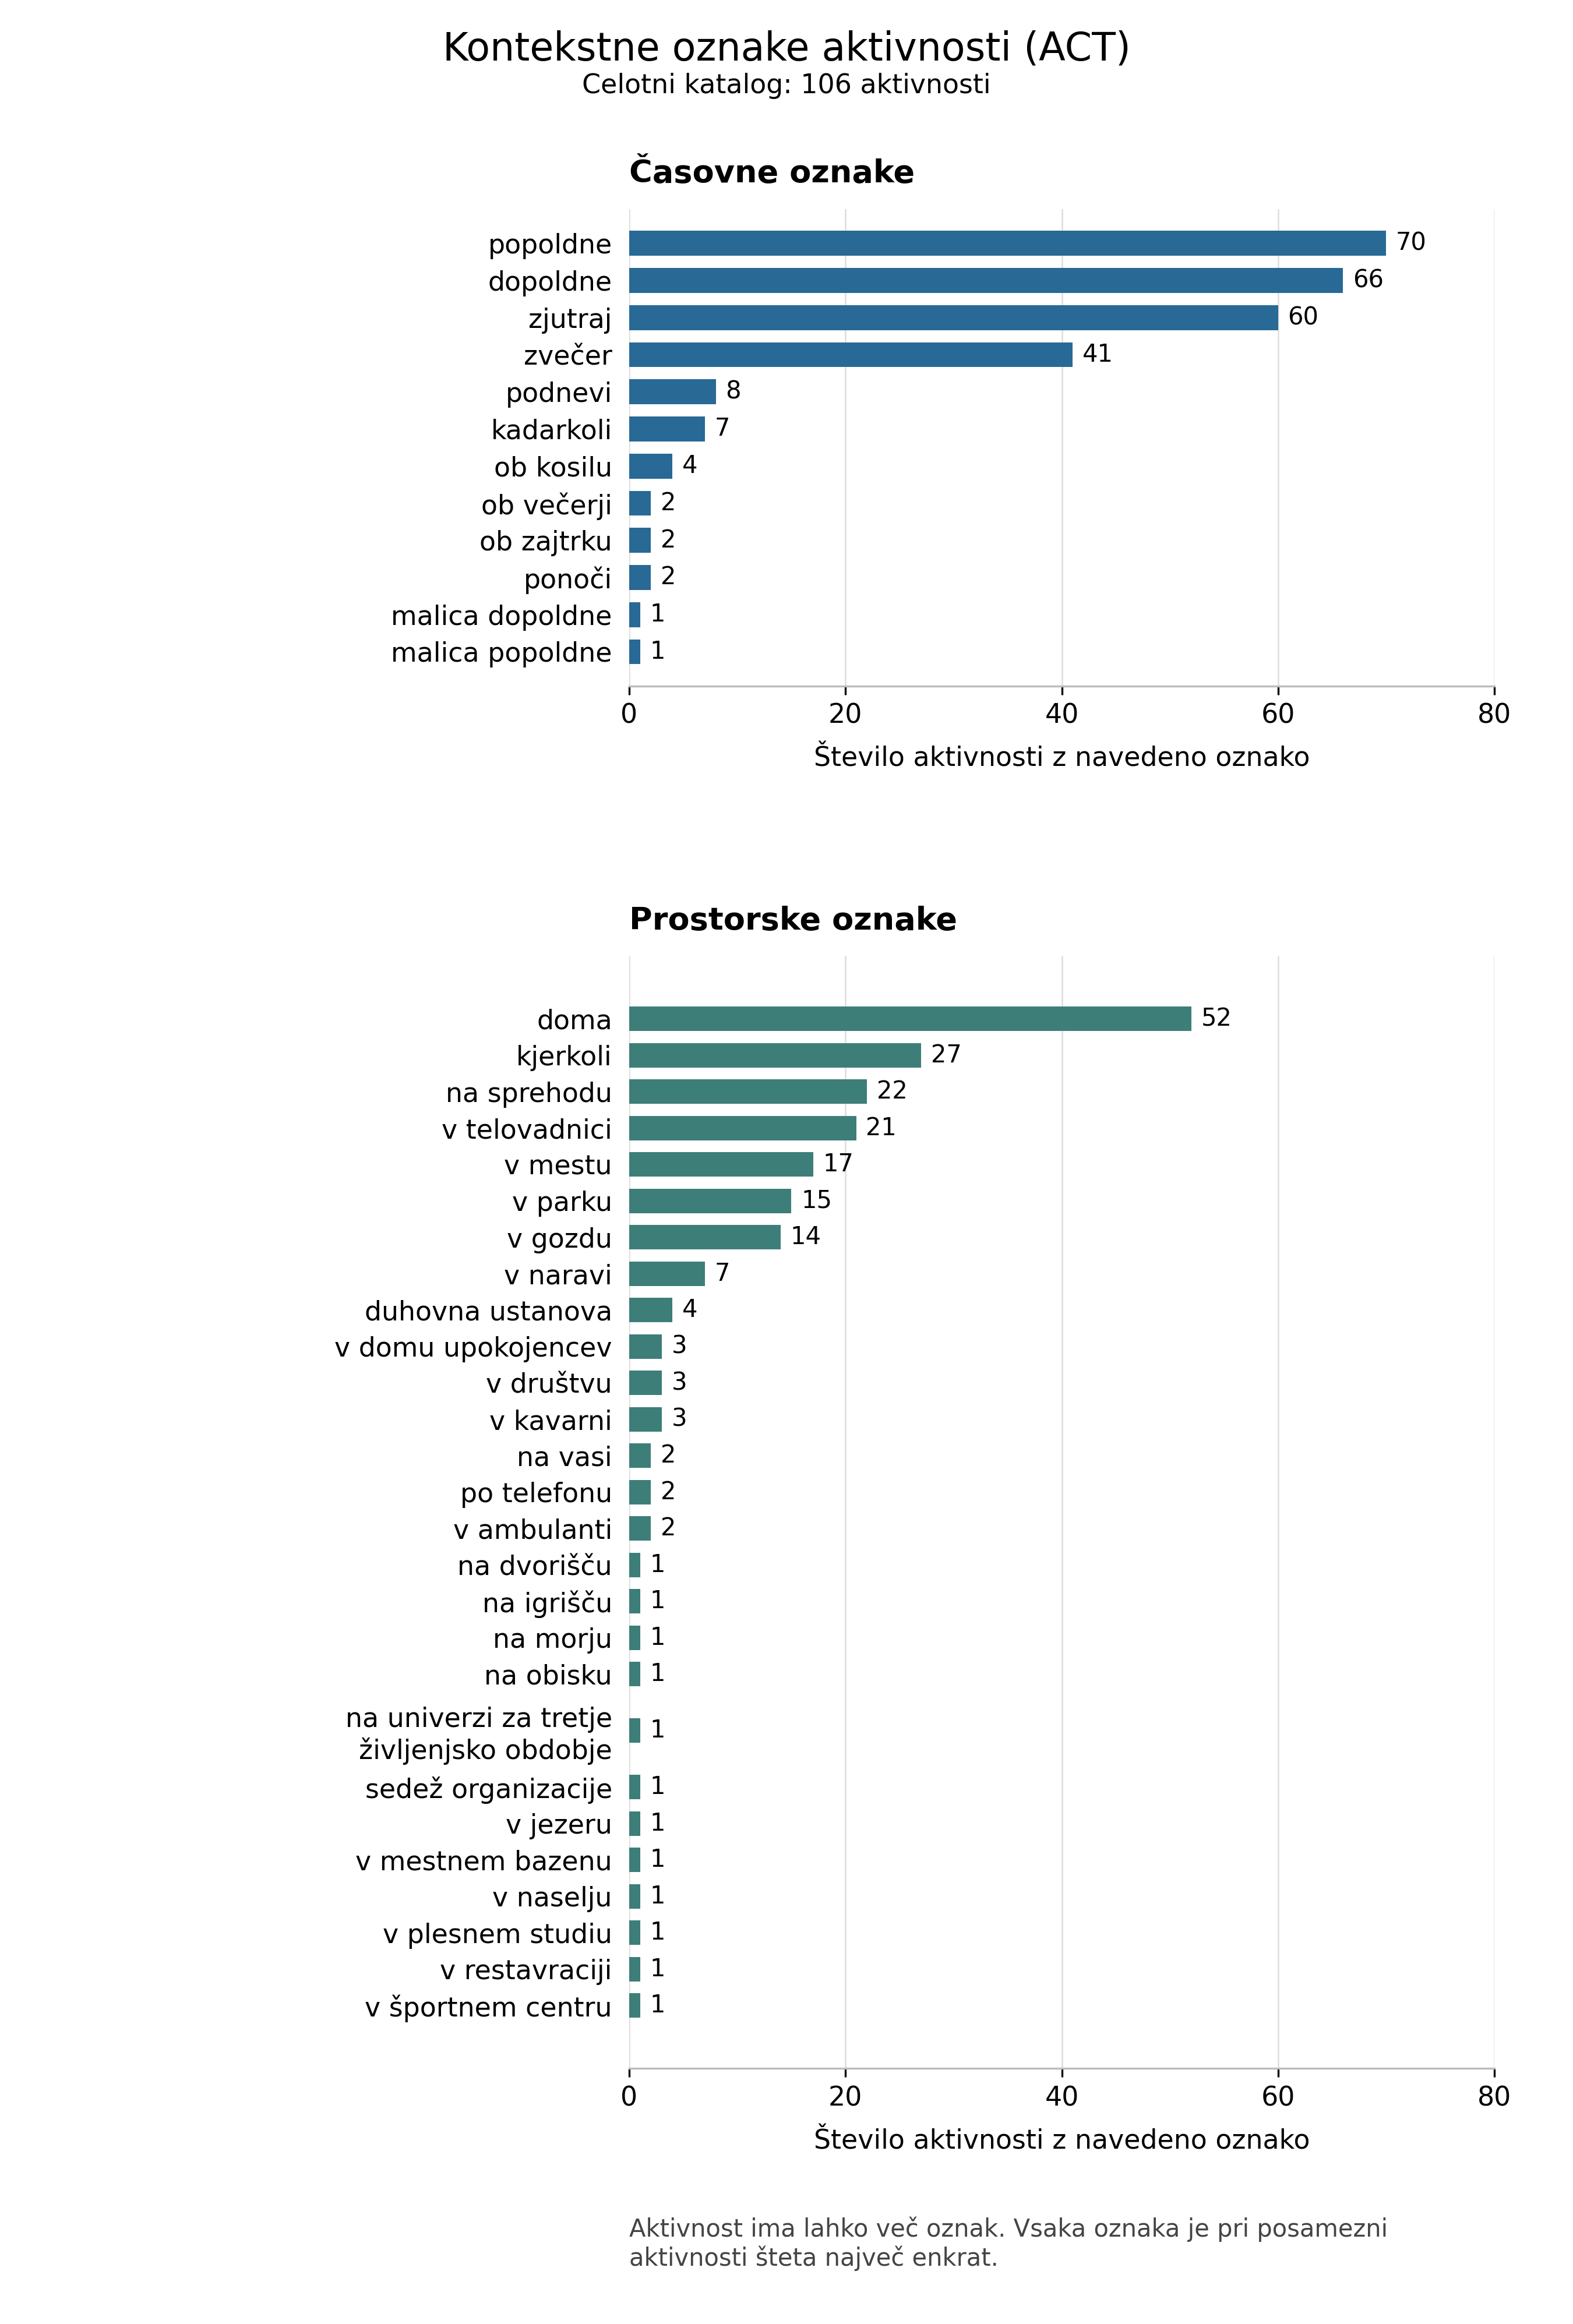
\includegraphics[height=0.78\textheight]
    {Slike/ContextGroup_hists_actC.png}
    \caption{Pogostost časovnih in prostorskih oznak ACT
    v katalogu 106 aktivnosti. Posamezna aktivnost ima
    lahko več oznak; vsaka oznaka je pri posamezni
    aktivnosti šteta največ enkrat.}
    \label{fig:hists_actC}
\end{figure}

\subsection{Opis segmentov M3, M4 in M5}
\label{sec:segments}

Skupine so določene na celotnem katalogu 106 aktivnosti, v eksperimentu
pa nastopa 34 aktivnosti vidika \texttt{activity}.
Tabela~\ref{tab:group_sizes} prikazuje, kako se po skupinah porazdelijo.
Navedene oznake ACT so najpogostejše pri uporabljenih aktivnostih;
posamezna aktivnost ima lahko več oznak.

\begin{table}[htbp]
\centering
\caption{Porazdelitev aktivnosti po skupinah M3, M4 in M5: celotni katalog
in 34 uporabljenih aktivnosti.}
\label{tab:group_sizes}
\footnotesize
\begin{tabular}{llrrp{6.4cm}}
\toprule
 & Skupina & Katalog & Uporabljene & Najpogostejše oznake uporabljenih \\
\midrule
M3 & 0 & 30 & 3 & dopoldne, popoldne; kjerkoli \\
   & 1 & 63 & 29 & zjutraj, dopoldne, podnevi; kjerkoli, v telovadnici, doma \\
   & 2 & 13 & 2 & zjutraj, dopoldne, popoldne; v gozdu, v mestu \\
\midrule
M4 & 0 & 33 & 8 & zjutraj, dopoldne; doma, v telovadnici \\
   & 1 & 29 & 2 & dopoldne, popoldne, zvečer; kjerkoli \\
   & 2 & 23 & 20 & podnevi, ob kosilu; kjerkoli \\
   & 3 & 21 & 4 & zjutraj, dopoldne, popoldne; različni kraji \\
\midrule
M5 & 0 & 12 & 2 & različni časi; v telovadnici \\
   & 1 & 32 & 9 & zjutraj, dopoldne; doma, v telovadnici \\
   & 2 & 21 & 19 & podnevi, ob kosilu; kjerkoli \\
   & 3 & 28 & 2 & dopoldne, popoldne, zvečer; kjerkoli \\
   & 4 & 13 & 2 & zjutraj, dopoldne, popoldne; v gozdu, v mestu \\
\bottomrule
\end{tabular}
\end{table}

Porazdelitev je zelo neenakomerna. Pri M3 je v skupini 1 kar 29 od
34 aktivnosti, zato je ta skupina skoraj enaka različici brez konteksta:
od njenih 3\,395 priporočil jih je 2\,782 (81,9~\%) enakih kot pri različici
brez konteksta. Pri M4 in M5 največja skupina vsebuje 20 oziroma
19 aktivnosti, predvsem prehranskih z oznako \emph{kjerkoli}.

\subsection{Vpliv segmentacije na uspešnost priporočilnega sistema}

Za kvantitativno primerjavo vpliva različnih plasti konteksta na uspešnost modela 
smo rezultate zbrali v Tabeli~\ref{tab:results_all_layers}. 

Primerjali smo naslednje pristope:

\begin{itemize}
    \item brez konteksta (baseline),
    \item razvrščanje po popularnosti in naključno rangiranje (pričakovana vrednost),
    \item s kontekstom (razdelek~\ref{sec:results_with_context}), z globalno in s kontekstno referenco,
    \item segmentacijo M3 (3 skupine),
    \item segmentacijo M4 (4 skupine),
    \item segmentacijo M5 (5 skupin).
\end{itemize}

\begin{table}[htbp]
\centering
\caption{Rezultati na testnih parih. Natančnost in priklic sta pri vseh vrsticah enaka F1. F1 z izen. upošteva izenačenja pri meji referenčnega seznama, povp. ref. ocena je povprečna testna ocena vrnjenih priporočil. Kontekstna referenca in M3--M5 uporabljajo ožje reference in niso neposredno primerljivi z globalno referenco.}
\label{tab:results_all_layers}
\footnotesize
\setlength{\tabcolsep}{4pt}
\begin{tabular}{lrrrr}
\toprule
Različica & F1 & F1 z izen. & Pokritost & Povp. ref. ocena \\
\midrule
Brez konteksta (baseline) & 0,339 & 0,982 & 1,000 & 3,066 \\
Popularnost (baseline) & 0,151 & 0,531 & 1,000 & 2,882 \\
Naključno (pričakovana vrednost) & 0,006 & 0,066 & 1,000 & 1,468 \\
S kontekstom, globalna ref. & 0,018 & 0,120 & 0,895 & 2,045 \\
Naključno s kontekstom, globalna ref. & 0,001 & 0,018 & 0,895 & 1,425 \\
S kontekstom, kontekstna ref. & 0,804 & 0,998 & 0,895 & 2,045 \\
Popularnost s kontekstom, kontekstna ref. & 0,718 & 0,907 & 0,895 & 1,942 \\
Naključno s kontekstom, kontekstna ref. & 0,532 & 0,653 & 0,895 & 1,425 \\
M3 (uteženo) & 0,623 & 0,988 & -- & 2,745 \\
M4 (uteženo) & 0,698 & 0,996 & -- & 2,280 \\
M5 (uteženo) & 0,682 & 0,997 & -- & 2,371 \\
\bottomrule
\end{tabular}

\end{table}


\begin{figure}[H]
\centering
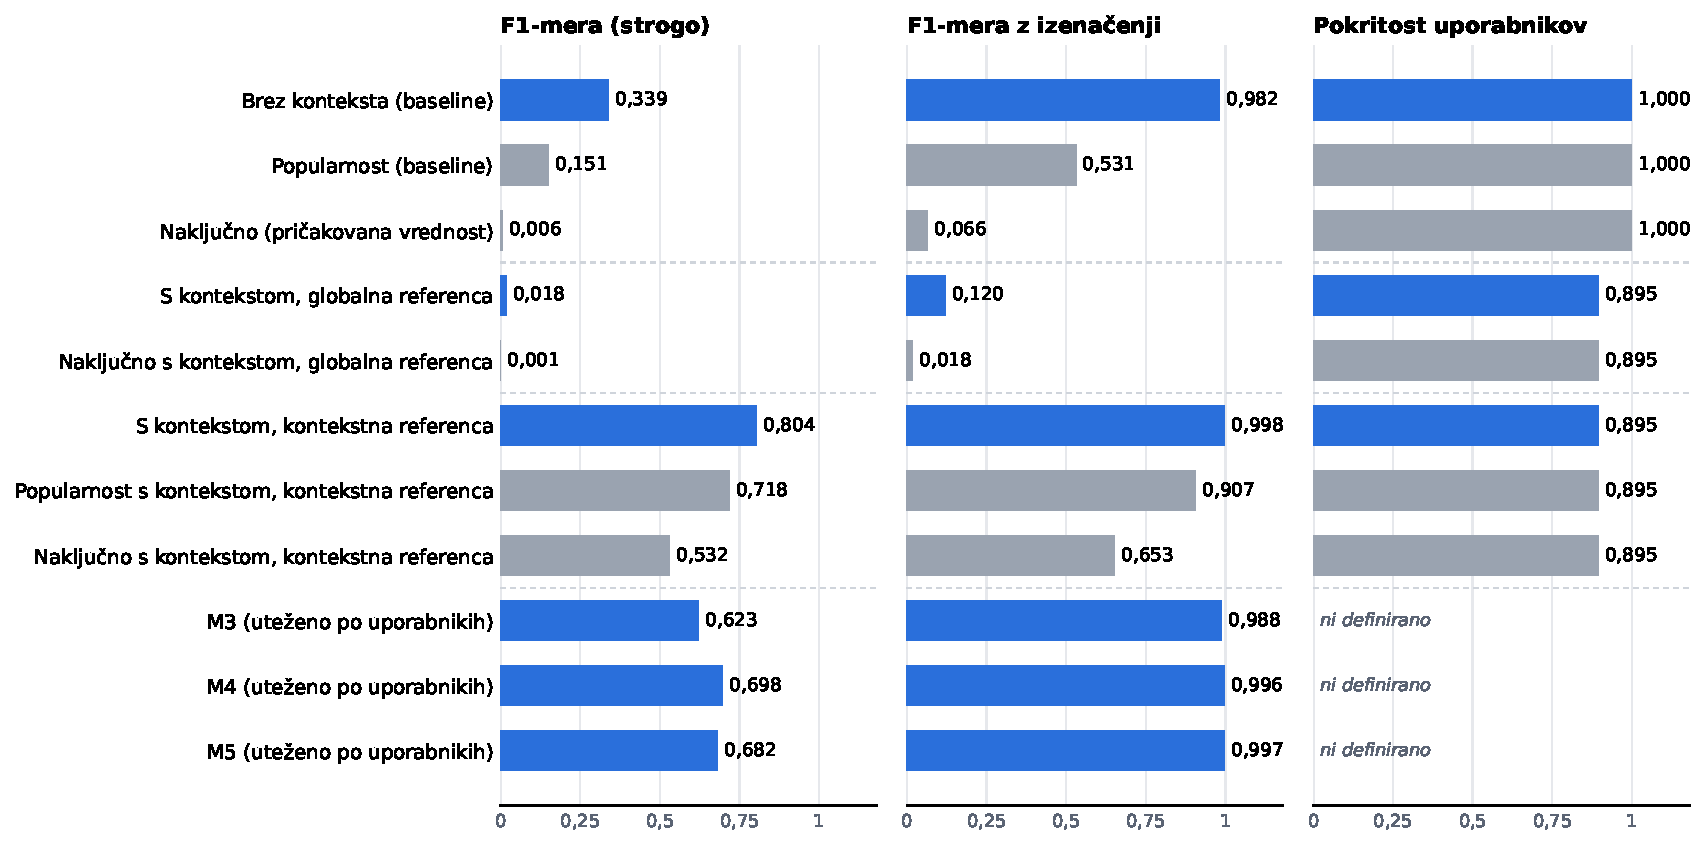
\includegraphics[width=\textwidth]{Slike/results_overview_20261125_222631.pdf}
\caption{Strogi F1, F1 z izenačenji in pokritost uporabnikov za vse različice
priporočanja (zagon 20261125\_222631). Sivi stolpci so primerjalne vrstice
(popularnost in pričakovana vrednost naključnega rangiranja).}
\label{fig:rezultati_metrike}
\end{figure}

Utežena povprečna F1-mera je znašala $0{,}623$
za M3, $0{,}698$ za M4 in $0{,}682$ za M5,
F1-mera z izenačenji pa $0{,}988$, $0{,}996$ in $0{,}997$.
Rezultati so prikazani tudi na Sliki~\ref{fig:rezultati_metrike}.

Priporočila so bila med skupinami porazdeljena neenakomerno.
Pri M3 so bila števila priporočil po skupinah
583, 3\,395 in 78, pri M4 3\,157, 291, 3\,234 in 513,
pri M5 pa 71, 3\,172, 3\,204, 291 in 78.

Majhne skupine dajejo trivialno F1-mero. V skupinah 0 in 2
pri M3, 1 pri M4 ter 0, 3 in 4 pri M5 ima vsak vključeni
uporabnik največ pet kombinacij, zato F1-mera znaša 1.
Skoraj enako velja za skupino 3 pri M4 ($0{,}996$).
Povprečje je zato uteženo po številu uporabnikov, vendar
majhne skupine vanj še vedno prispevajo. Pri največjih
skupinah, to je 1 pri M3, 2 pri M4 in 2 pri M5, F1-mera
znaša $0{,}378$, $0{,}357$ in $0{,}366$.

\subsection{Razprava}

Skupinsko filtriranje omeji izbor na kombinacije aktivnosti
iz iste skupine. Model SVD se pri tem ne uči ponovno,
zato segmentacija ne spreminja napovedi ocen, temveč samo izbor
priporočil in referenčne množice. Te se razlikujejo med skupinami
in različicami, zato vrednosti ne sestavljajo lestvice uspešnosti.


\chapter{Zaključki in razprava} \label{chap:discussion_conclusion}
V magistrskem delu smo razvili priporočilni sistem za
kombinacije dnevnih aktivnosti starejših uporabnikov.
Model SVD napoveduje ocene kombinacij, kontekst pa se
upošteva z naknadnim filtriranjem. Posamezna kombinacija
vsebuje od ene do treh aktivnosti in ne določa njihovega
časovnega razporeda.

Vrednotenje je bilo izvedeno na naboru 3\,053\,029
izračunanih ocen za 679 uporabnikov in 6\,579 kombinacij.
Primerjava algoritmov in izbira hiperparametrov sta
potekali na razvojnem delu podatkov, končno vrednotenje
pa na ločenem testnem delu.
Med primerjanimi konfiguracijami je SVD dosegel
najnižjo povprečno razvojno RMSE.
Končni model z izbranimi hiperparametri je na
odloženem testnem delu dosegel RMSE $0{,}0819$,
MAE $0{,}0531$ in FCP $0{,}9966$.

Pri izboru petih priporočil brez konteksta je povprečna
F1-mera znašala $0{,}339$, z izenačenji $0{,}982$, pri razvrščanju
po popularnosti pa $0{,}151$. Sistem je vrnil pet priporočil
vsakemu uporabniku. Kontekstno filtriranje je število
priporočil zmanjšalo s 3\,395 na 2\,534, priporočila
pa je prejelo 608 od 679 uporabnikov.
F1-mera kontekstne različice je znašala
$0{,}018$ z globalno in $0{,}804$ s kontekstno referenco.
Na 398 uporabnikih z več kot petimi skladnimi testnimi kombinacijami,
pri katerih izbor ni trivialen, je SVD s kontekstno referenco dosegel
$0{,}700$, razvrščanje po popularnosti $0{,}569$, naključno rangiranje
pa pričakovano $0{,}285$. Model torej tudi znotraj kontekstno skladnih
kombinacij razvršča bolje od obeh primerjav.

Pri različicah M3, M4 in M5 so bila priporočila
vrednotena znotraj posameznih skupin.
Po uporabnikih utežene F1-mere so znašale $0{,}623$, $0{,}698$
in $0{,}682$. Skupine so zelo neenakomerne: največja pri M3 vsebuje
29 od 34 aktivnosti in je skoraj enaka različici brez konteksta, v majhnih
skupinah pa je F1-mera trivialno 1.

Rezultati kažejo razliko med napovedovanjem izračunanih
ocen in zagotavljanjem priporočil v določenem kontekstu.
Model doseže nizko napako ocen, strogi filter pa
kljub temu pri 71 od 679 uporabnikov (10,5~\%) izloči vse
kandidatne kombinacije; pri 48 od njih skladne kombinacije ni
niti v celotnem naboru. Napovedovanje ocen
in obravnavo konteksta je torej mogoče izvajati ločeno, pri čemer
naknadno filtriranje ne zagotavlja polnih seznamov priporočil.

\section{Omejitve}
\label{sec:limitations}

\paragraph{Izvor ocen.}
Učne in referenčne ocene so izračunane z istim pravilom iz vprašalniških
odgovorov, uteži in združljivosti aktivnosti ter niso ocene zadovoljstva
uporabnikov. Rezultati zato merijo, kako dobro model povzame uporabljeno
pravilo, in ne uporabnosti priporočil; ocene bi bilo mogoče izračunati tudi
neposredno. Model SVD v tem delu predstavlja ogrodje, uporabno tudi pri
dejanskih uporabniških ocenah. Izpis latentnih faktorjev sam po sebi
ni uporabniku razumljiva razlaga priporočila.

\paragraph{Izenačenja.}
Posamezen uporabnik ima največ šest različnih ocen, zato so izenačenja na meji
top-5 pogosta (658 od 679 uporabnikov). Pri osnovni različici je imelo
97,3~\% priporočil zunaj referenčne množice enako referenčno oceno kot
njen peti element. Stroga F1-mera zato odraža tudi leksikografsko razreševanje
izenačenj, F1-mera z izenačenji pa je visoka, ker model dobro povzame
pravilo. Tudi brezhibna napoved ocen bi ob naključnem razreševanju
izenačenj dosegla pričakovano strogo F1-mero le $0{,}321$.
Izenačenja so prisotna tudi v referenčnih množicah skupin.

\paragraph{Različne referenčne množice.}
Kontekstna referenca in reference skupin M3--M5 so ožje od globalne in
vključujejo različne množice uporabnikov, zato višja F1-mera kontekstnih
in skupinskih različic ne pomeni, da kontekst izboljša sistem. Pri
210 uporabnikih z največ petimi skladnimi kombinacijami in pri majhnih
skupinah je F1-mera trivialno 1.

\paragraph{Simuliran kontekst.}
Konteksti so vzorčeni neodvisno in enakomerno iz oznak aktivnosti in
ne opisujejo dejanskih okoliščin uporabnikov. Oznake se primerjajo
dobesedno, pripadnosti skupinam M3--M5 pa so prevzete iz kataloga.

\paragraph{Pravilo ocenjevanja.}
Ker se prispevki aktivnosti
seštevajo, kazen za nezdružljivost pa je ne glede na število nezdružljivih parov enaka 1, ima trojka
z nezdružljivim parom, pri kateri so vsi trije odgovori pritrdilni, pri uteži $s_u^{(g)} > 1$
višjo oceno kot združljiv par s pritrdilnima odgovoroma ($3s_u^{(g)} - 1 > 2s_u^{(g)}$). Med 3\,395
priporočili brez konteksta je 3\,327 trojk, 1\,773 (52~\%) pa jih vsebuje vsaj en nezdružljiv par.
Med 2\,534 priporočili s kontekstom vsebuje nezdružljiv par 1\,861 (73~\%) kombinacij, 171 (6,7~\%)
pa isto aktivnost dvakrat pod različnima identifikatorjema (vprašanji \texttt{Ac\_AB4\_1} in
\texttt{Ac\_AB4\_8}). Del kombinacij vsebuje tudi aktivnosti, pri katerih je uporabnik na pripadajoče
vprašanje odgovoril z 0 (11,6~\% brez konteksta in 55,1~\% s kontekstom); v kombinacijo pridejo
zaradi drugih članov. Visoko ujemanje s pravilom zato ne zagotavlja vsebinsko smiselnih kombinacij.

\paragraph{Izbira hiperparametrov.}
Vse štiri izbrane vrednosti hiperparametrov so na robu preizkušene mreže
(150 faktorjev, 30 epoh, učna hitrost $0{,}005$, regularizacija $0{,}02$),
zato je optimum lahko zunaj nje. Ostali trije algoritmi niso bili
prilagajani.

\section{Nadaljnje delo}

Smiselno nadaljnje delo je preverjanje priporočil
z domenskimi strokovnjaki oziroma uporabniki,
presoja kontekstnih pravil glede na dejanske
okoliščine uporabe ter presoja pravila ocenjevanja, predvsem
obravnave nezdružljivih in podvojenih aktivnosti.

\cleardoublepage\phantomsection\addcontentsline{toc}{chapter}{Literatura} % vnos literature v kazalo
\bibliographystyle{ieeetrslo}
\bibliography{literatura}

\end{document}
%%%%%%%%%%%%%%%%%%%%%%%%%%%%%%%%%%%%%%%%%%%%%%%%%%%%%%%%%%%%%%%%%%%%%%%%%%%%%%%%%%%%%%%%%%%%%%%%%%%%%%%%%%%%%%%%%%%%%%%%
